\fenicschapter{Turbulent flow and fluid--structure interaction}
              {Turbulent flow and fluid--structure interaction}
              {Johan Hoffman, Johan Jansson, Niclas Jansson, Claes Johnson and Rodrigo Vilela De Abreu}
              {hoffman-1}

The FEniCS project aims towards the goals of
generality, efficiency, and simplicity, concerning
mathematical methodology, implementation, and
application, and the Unicorn project is an
implementation aimed at FSI and high Re turbulent flow
guided by these principles. Unicorn is based on the
DOLFIN/FFC/FIAT suite and the linear algebra package
PETSc, and we here present some key elements of
Unicorn, and a set of computational results from
applications. The details of the Unicorn
implementation is described in
Chapter~\ref{chap:hoffman-2}.

\section{Background}

For many problems involving a fluid and a structure,
decoupling the computation of the two is not feasible
for accurate modeling of the phenomenon at hand,
instead the full fluid--structure interaction (FSI)
problem has to be solved together as a coupled
problem. This includes a multitude of important
problems in biology, medicine and industry, such as
the simulation of insect or bird flight, the human
cardiovascular and respiratory systems, the human
speech organ, the paper making process, acoustic noise
generation in exhaust systems, airplane wing flutter,
wind induced vibrations in bridges and wave loads on
offshore structures. Common for many of these problems
is that for various reasons they are very hard or
impossible to investigate experimentally, and thus
reliable computational simulation would open up for
detailed study and new insights, as well as for new
important design tools for construction.

Computational methods for FSI is a very active
research field today. In particular, major open
challenges of computational FSI include: (i)
robustness of the fluid--structure coupling, (ii) for
high Reynolds numbers (Re) the computation of
turbulent fluid flow, and (iii) efficiency and
reliability of the computations in the form of
adaptive methods and quantitative error estimation.

\section{Simulation of high Re turbulent flow}

The focus of Unicorn is high Re turbulent fluid flow, also including fluid--structure interaction. Direct numerical simulation (DNS) of turbulent flow is limited to moderate Re and simple geometry, due to the high computational cost of resolving all turbulent scales in the flow. The standard e.g. in the automotive industry is simulation based on Reynolds averaged Navier-Stokes equations (RANS), where time averages (or statistical averages) are computed to an affordable cost, with the drawback of introducing turbulence models based on parameters that have to be tuned for particular applications.

An alternative to DNS and RANS is Large eddy simulation (LES) \cite{Sagaut2005}, where a filter is applied to the Navier-Stokes equations to derive a new set of equations with a smallest scale given by the filter width, and where the effect of the filter is the introduction of so called subgrid stresses which need to be modeled in a subgrid model. A subgrid model can be motivated by physics theory or experiments, and the main effect of the subgrid model is to dissipate kinetic energy, for example in the form of turbulent viscosity.

Typically the numerical method used to approximate the LES equations also introduces dissipation, and thus there are two sources of kinetic energy dissipation; the subgrid model and the numerical method. One class of methods, Implicit LES (ILES), relies completely on the numerical method to act as subgrid model, without any additional explicit subgrid model \cite{Sagaut2005}. Turbulence simulation in Unicorn is based on ILES in the form a stabilized finite element method, referred to as a General Galerkin (G2) simulation \cite{HoffmanJohnson2007}, where a least squares stabilization based on the residual of the Navier-Stokes equations acts a an ILES subgrid model.

More specific, in the current G2/ILES implementation of Unicorn continuous piecewise linear approximation is used in space and time, together with a least squares stabilization based on the residual \cite{HoffmanJohnson2007}.

\section{Turbulent boundary layers}
\label{section:blayer}

The choice of boundary conditions at a solid wall is critical for accurate LES modeling of fluid flow, in particular to capture flow separation phenomena. In Unicorn, laminar boundary layers are fully resolved by the computational method by applying no slip (zero velocity) boundary conditions at the wall. On the other hand, computational resolution of turbulent boundary layers is only possible at limited Reynolds numbers and for simple geometries.

The standard way to model the effect of turbulent boundary layers is to divide the computational domain into: (i) an interior part $\Omega$, and (ii) a boundary layer region. In the boundary layer a simplified model of the flow is used to provide boundary conditions to the LES equations to be solved in the interior part $\Omega$. Boundary conditions are typically in the form of a wall shear stress, and the coupling between (i) and (ii) may be one-way from (ii) to (i), or more closely coupled. Wall shear stress models are developed based on experimental data, theory, or computation by a simplified model (e.g. a RANS model). For an overview of boundary layer modeling, see e.g. \cite{SagautDeckTerracol2006,PiomelliBalaras2002}.

The wall shear stress model in Unicorn takes a similar form as the simple Shumann model \cite{Schumann1975}, with the tangential velocity proportional to the local wall shear stress through a skin friction parameter (or function) $\beta$. That is, the following boundary conditions are used for the velocity $u$ and stress $\sigma$:
\begin{eqnarray}
&&u\cdot n=0, \label{slfra} \\
&&\beta u\cdot \tau _k + n^T\sigma \tau _k=0,\quad k=1,2, \label{slfrb}
\end{eqnarray}
for  $(x,t)\in \Gamma_{solid}\times [0,T]$, with $n=n(x)$ an outward unit normal vector, and $\tau_k=\tau_k(x)$ orthogonal unit tangent vectors of $\Gamma_{solid}$. Matrix notation is used, with all vectors $v$ being column vectors and the corresponding row vector is denoted $v^T$. The non-penetration boundary condition is applied strongly, whereas a weak implementation is used for the wall shear stress boundary condition.

\section{Adaptivity and a posteriori error estimation}

A posteriori error estimation involves only computable quantities, which opens for adaptive methods with quantitative error control. The basic idea of adaptive algorithms is to optimize the computational method with respect to the goal (output of interest) of the computation. Typical parameters of an adaptive finite element method include the local mesh size (h-adaptivity), local degree of the finite element approximation (p-adaptivity), local shape of the cells (r-adaptivity), or combinations thereof. Other possible parameters may be the time step size and the stabilization parameters.

In Unicorn, an approach to a posteriori error estimation is used where the error in a chosen output quantity can be estimated in terms of the solution of an associated linearized dual problem. The basic framework is described e.g. in the survey articles \cite{ErikssonEstepEtAl1995,BeckerRannacher2001,GilesSuli2002}.

Using standard techniques of a posteriori error analysis, an a posteriori error estimate for G2 can be derived in the following form:
\begin{equation}
\vert M(u) - M(U) \vert \leq \sum_K {\cal E}_K
\end{equation}
with $M(u)$ the target output to compute and $M(U)$ the approximation, with $U$ a G2 solution, and ${\cal E}_K$ a local error indicator for cell $K$.
The error indicator ${\cal E}_K$ is constructed from the residual, measuring local errors,
weighted by the solution to a dual (adjoint) problem measuring the effect of local errors
on the output $M(\cdot)$. The implementation of the dual problem in Unicorn is based on the cG(1)cG(1) method described in \cite{HoffmanJohnson2007}. The computational mesh is then modified according to $ {\cal E}_K$, by mesh refinement, coarsening or smoothing.

Adaptive G2 methods (also referred to as Adaptive DNS/LES) have been used in a number of turbulent flow computations to a very low computational cost \cite{Hoffman2005,HoffmanJohnson2006b,Hoffman2006,Hoffman2009,HoffmanJansson2009,VilelaJanssonEtAl2010}, where convergence is obtained in output quantities such as drag, lift and pressure coefficients and Strouhal numbers, using orders of magnitude fewer numbers of mesh points than with LES methods based on ad hoc refined computational meshes in the literature.

\section{Robust fluid--structure coupling}

In a computational method based on so called weakly coupled FSI, separate solvers can be used for the fluid and the structure, with the benefit of being able to reuse existing dedicated fluid and structure solvers. To couple the fluid and the structure, boundary data such as displacements and stresses is exchanged over the fluid--structure interface, either as part of a fixed-point iteration or in a fully explicit fashion. To make the coupling more robust the equations for the fluid and the structure can be placed in the same algebraic system together with all coupling conditions, corresponding to a so called strong FSI coupling.

Another approach is to formulate the fluid and the structure as one single continuum model, which is then said to be a monolithic FSI method. In Unicorn a monolithic method is used referred to as Unified Continuum FSI (UC-FSI) \cite{HoffmanJanssonStockli2011}, where the fluid and the structure are discretized by the same finite element method over the combined fluid--structure continuum. A velocity formulation is used for the structure to make it consistent with the corresponding fluid equations, and the FSI problem thus takes the form of a multiphase flow problem, with the two phases, the fluid and the structure, described by different constitutive laws. In particular, coupling conditions for displacements and stresses are directly satisfied when using a continuous finite element discretization, which makes UC-FSI very robust.

The computational mesh is made to follow the deformation of the structure, and in the fluid part mesh smoothing is used to optimize the mesh quality, corresponding to an ALE method for the combined fluid--structure continuum.
In Unicorn, UC-FSI is implemented based on a continuous piecewise linear approximation in space and time, and a simple streamline diffusion stabilization is used, similar to the method in \cite{Hansbo2000}.
See \cite{HoffmanJanssonStockli2011} for details on the method.

\section{Applications}

In this section the capability of the Unicorn solver is illustrated by a set of simulation results, connecting to the main focus described above of high Re turbulent flow and robust fluid structure interaction. Quantitative results are presented for benchmark problems of turbulent flow and FSI, and qualitative results for a turbulent flow FSI problem is presented where no reference data is available. A sensitivity study is also presented, where the skin friction parameter of the boundary layer model is varied to observe the effect on flow separation.

\subsection{High Re turbulent flow}

Unicorn implements the computational method used for turbulent flow simulation in \cite{Hoffman2005,HoffmanJohnson2006b,Hoffman2006,Hoffman2009,HoffmanJansson2009,VilelaJanssonEtAl2010}.
To illustrate the basic features of this method we consider the simple benchmark problem to compute a time average of the drag force on a cube. Starting from a very coarse tetrahedral mesh with 17~952 vertices, the mesh is adaptively refined 17 times, in each iteration marking 10\% of the tetrahedrons in the mesh for refinement by bisection. In Fig.\ref{fig:cube1} the corresponding drag coefficient is shown as the mesh is refined, converging to a value of $c_D\approx 1.25\pm 5\%$ over the time interval chosen in the computation. Computing the drag coefficient over a longer time interval would give better confidence in the mean value, at a higher computational cost. In \cite{Mccormick1995} an interval of $1.0-1.2$ is given for the drag coefficient $c_D$, although the detailed setup of the underlying experiments is not clear. We note that for this case when flow separation is given by the sharp corners of the geometry, $c_D$ is considered independent of the specific (high) Reynolds number \cite{Mccormick1995}.
We conclude that the Unicorn results are consistent with experimental findings.

In Fig.\ref{fig:cube2} snapshots of the solution is shown for the adaptively refined mesh, and in
Fig.\ref{fig:cube3} a snapshot of the gradient of the dual solution is shown which provides sensitivity information with respect to the computation of drag force. Where this gradient is large, local computational errors must be made small by refining the mesh, since the error in drag is given by the product of the gradient of the dual solution and local errors, expressed as residuals weighted by the local mesh size. I Fig.\ref{fig:cube3} a snapshot of such a local error is shown, where we note that this local error is reduced where the gradient of the dual solution is large but left large in other areas.

Two main features of the adaptive method are: (i) a converged approximation of the drag coefficient $c_D$ (within 5\%) is obtained using very few degrees of freedom, and (ii) the mesh is automatically constructed from a coarse mesh, thus bypassing the cost and challenge of ad hoc mesh design. A full discussion of these computations is available in \cite{HoffmanJansson2011}.


\begin{figure}
\centering
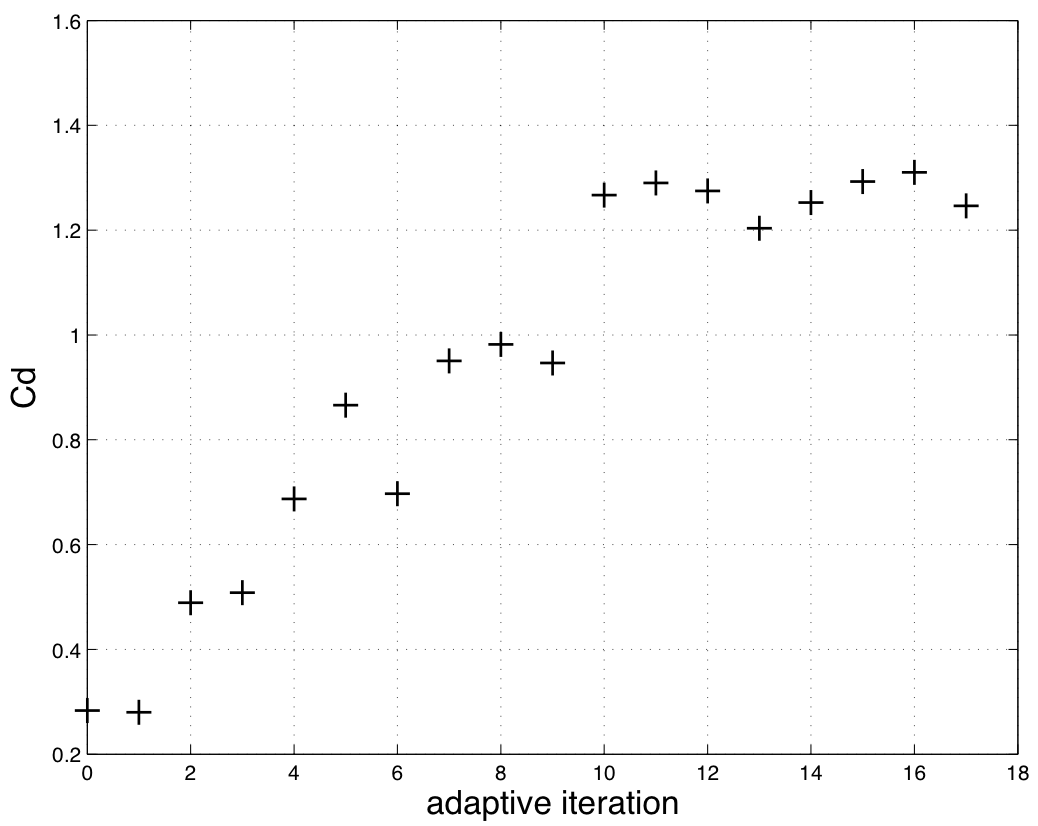
\includegraphics[height=5.4cm]{chapters/hoffman-1/png/fig1a.png}
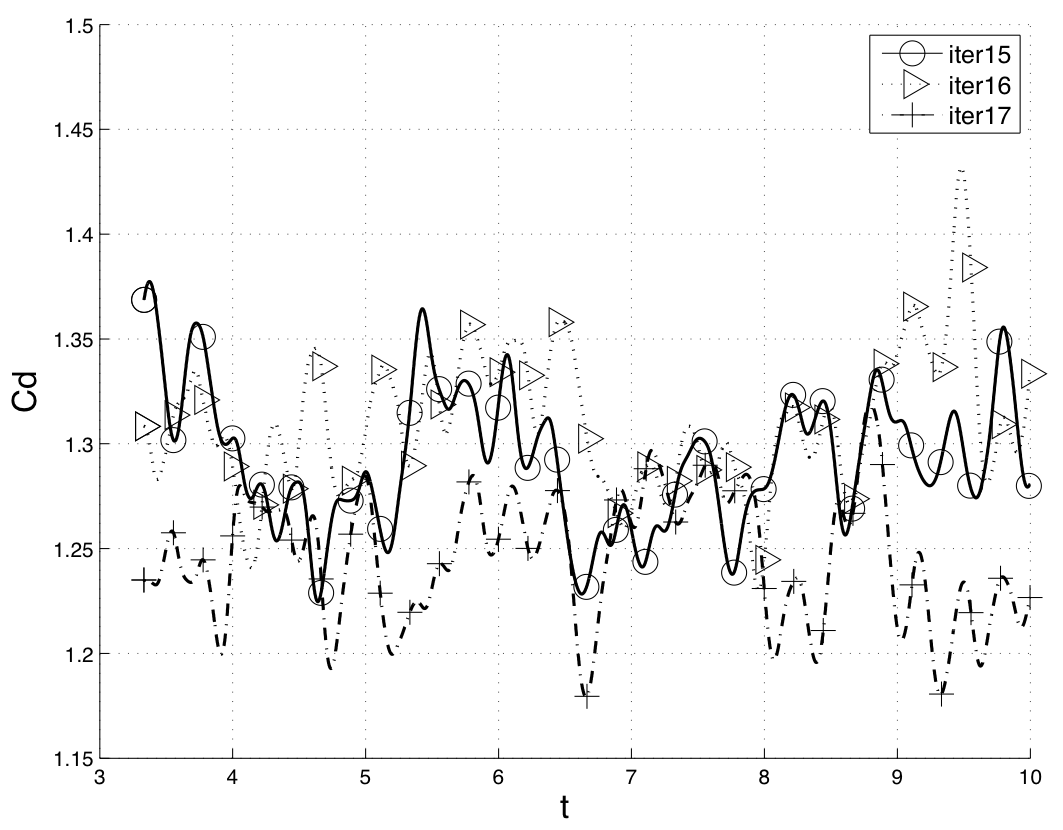
\includegraphics[height=5.4cm]{chapters/hoffman-1/png/fig1b.png}
\caption{Flow around a cube: convergence of the drag coefficient under mesh refinement.}
\label{fig:cube1}
\end{figure}

\begin{figure}
\centering
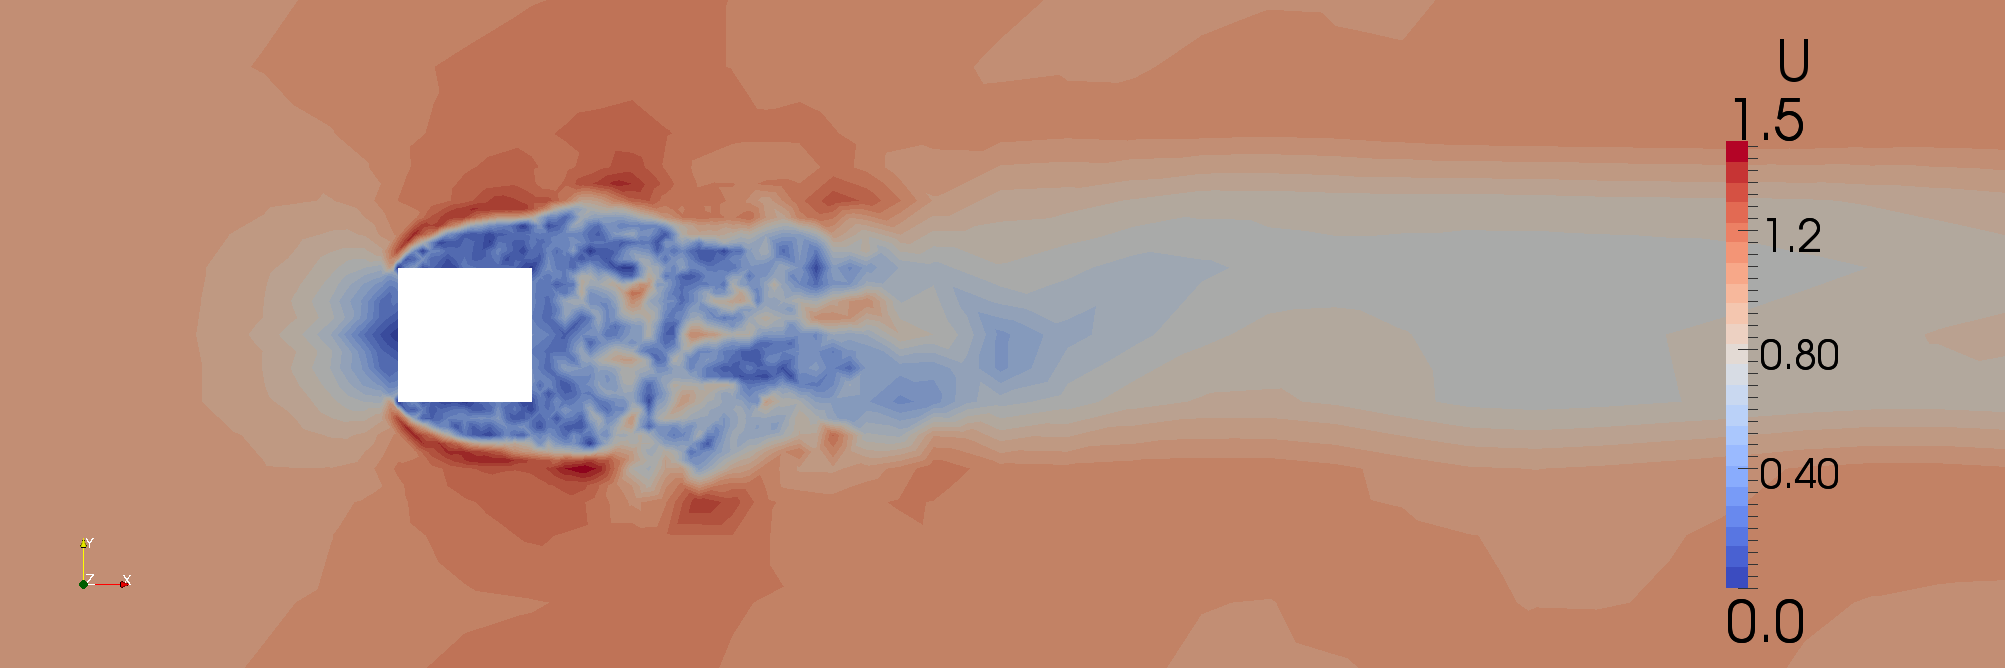
\includegraphics[width=11cm]{chapters/hoffman-1/png/fig2b.png}

\medskip

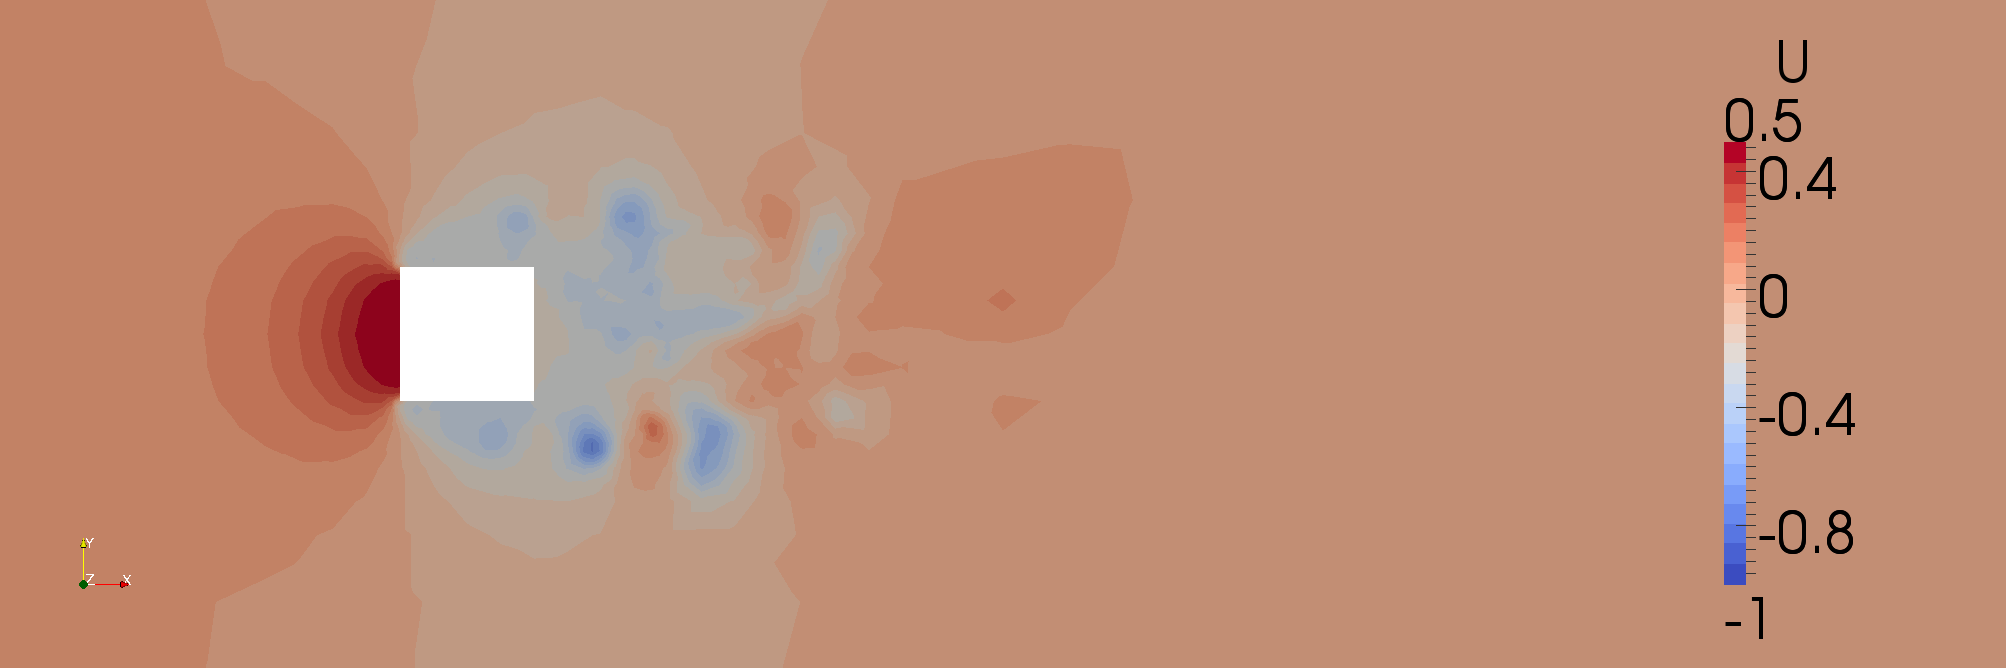
\includegraphics[width=11cm]{chapters/hoffman-1/png/fig2c.png}
\caption{Flow around a cube: snapshots of velocity (upper) and pressure (lower) for the finest mesh.}
\label{fig:cube2}
\end{figure}

\begin{figure}
\centering
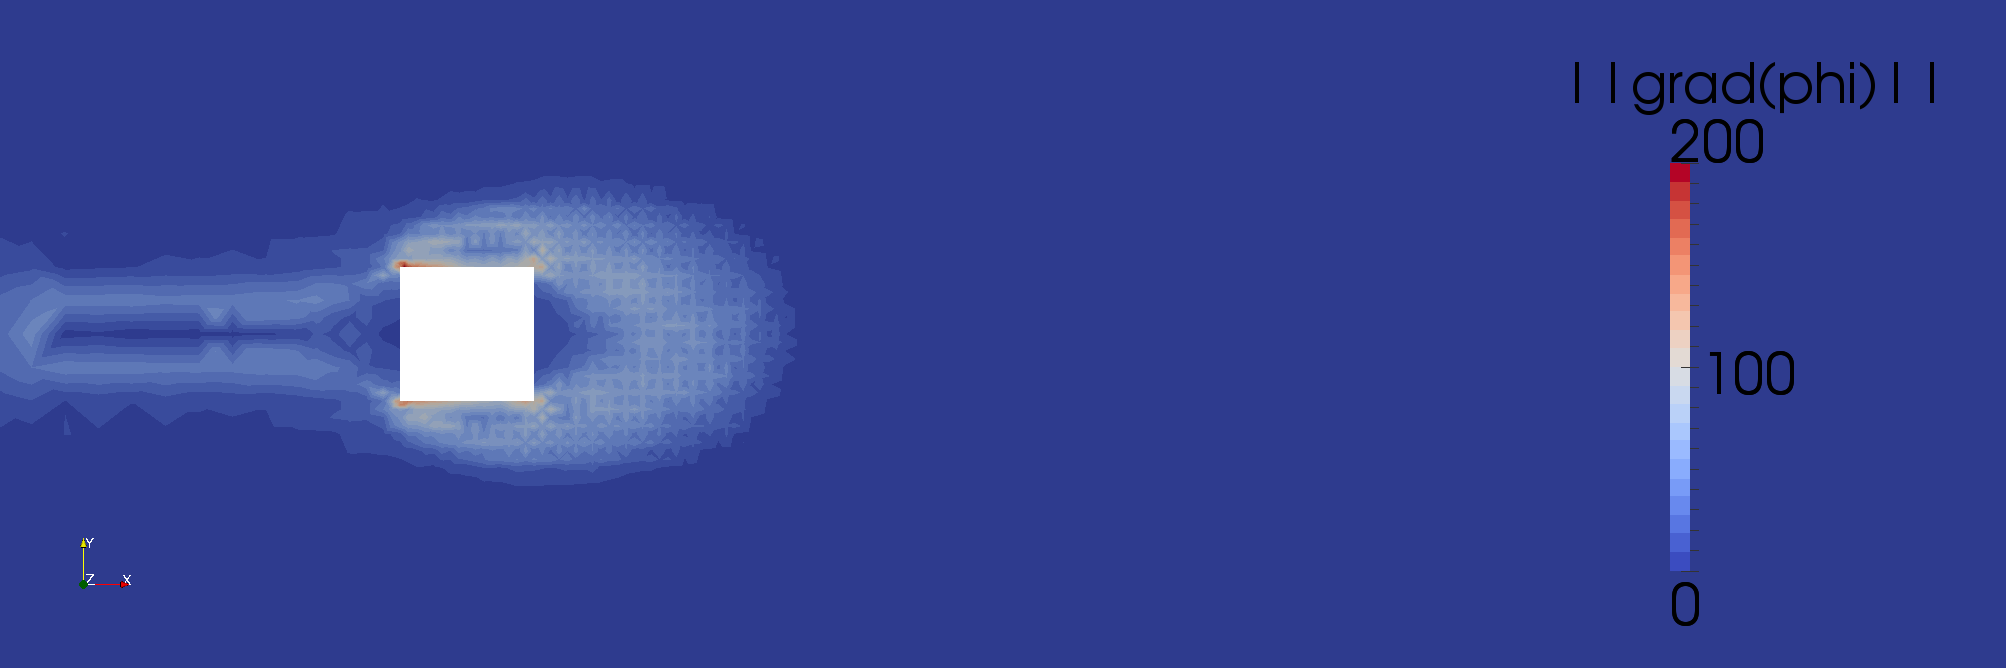
\includegraphics[width=11cm]{chapters/hoffman-1/png/fig3a.png}

\medskip

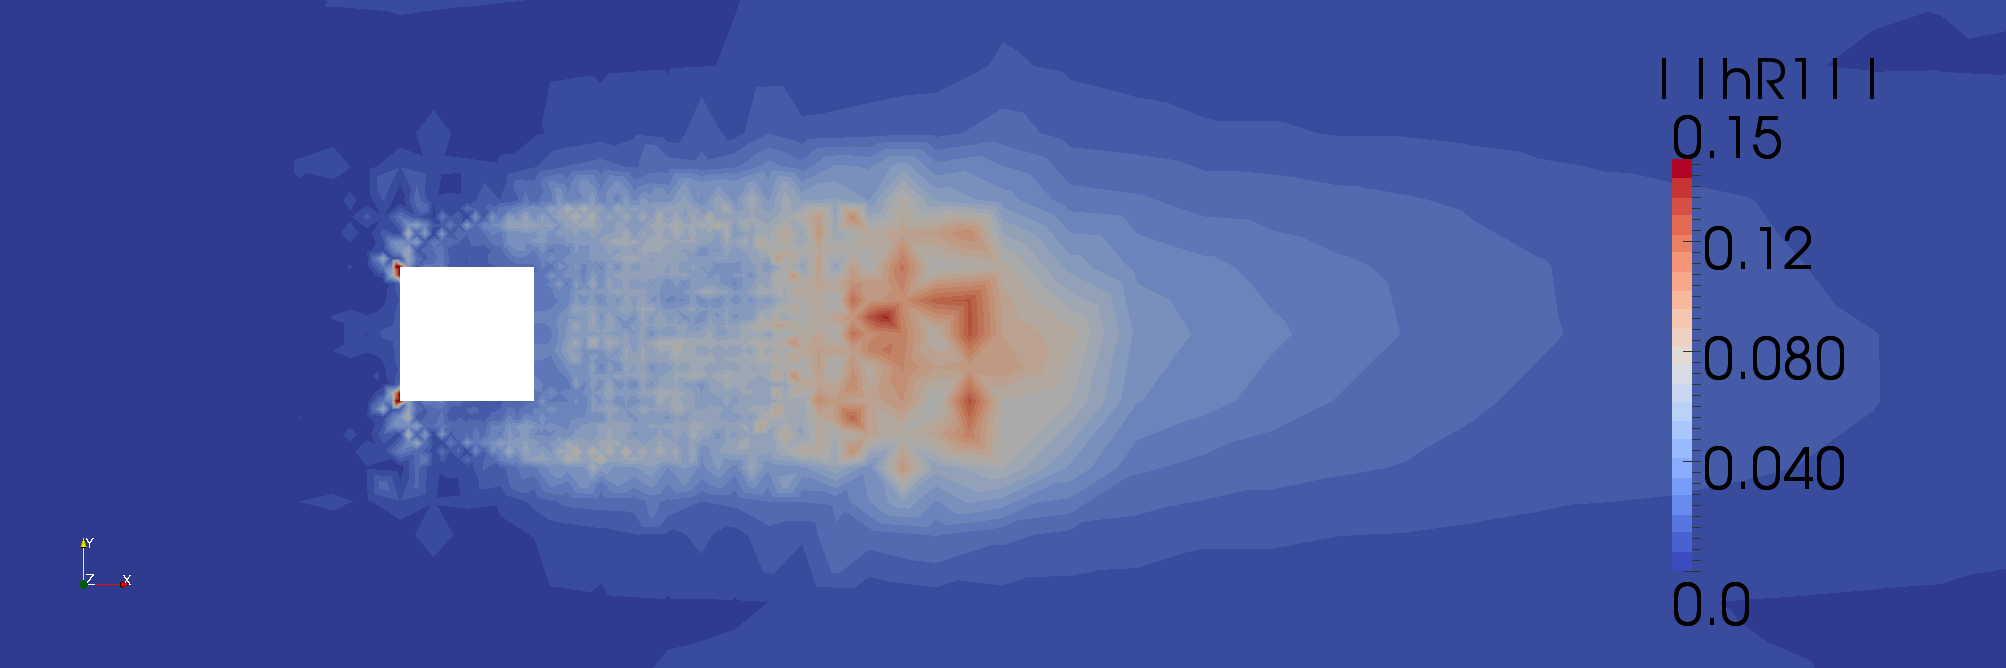
\includegraphics[width=11cm]{chapters/hoffman-1/png/fig3b.png}
\caption{Flow around a cube: gradient of dual velocity (upper) and local error (lower), on a mesh after 16 adaptive mesh refinements.}
\label{fig:cube3}
\end{figure}


\subsection{Turbulent flow separation}

In Unicorn, the effect of turbulent boundary layers is modeled by a skin friction wall shear stress model, described above. This model has one parameter $\beta$, which is related to the skin friction stress (following \cite{Schumann1975} a skin friction stress normalized by a velocity). Higher Reynolds number is modeled by a smaller $\beta$, based on experimental observation that the skin friction (coefficient) decrease with increasing $Re$.

To estimate the dependence of the computational result on $\beta$, in \cite{HoffmanJansson2009} a computational study carried out using Unicorn, where the drag force of a circular cylinder is computed adaptively based on a posteriori error estimation. In particular, the phenomenon of drag crisis is targeted, characterized by a sudden drop in the non-dimensional drag coefficient for a cylinder for $Re$ increasing beyond a critical size of about $10^5$. By decreasing the skin friction parameter $\beta$, modeling an increasing $Re$, the drag crisis scenario is reproduced using Unicorn, in agreement with the high $Re$ experimental data available in the literature \cite{Zdravkovich2003}. In particular, the drag coefficient drops to a level found in experiments after drag crisis, and 3D so called cell structures develop in the form of streamwise vorticity, also reported in the literature \cite{Zdravkovich2003}.
For vanishing skin friction the flow approaches a state independent of the skin friction parameter, which thus corresponds to a free slip boundary condition, see Fig.\ref{fig:1}-\ref{fig:3}. Although controversial, this suggests a dominant inviscid separation mechanism independent of the boundary layer, investigated in \cite{HoffmanJohnson2008b,HoffmanJansson2009}.


\begin{figure}
\centering
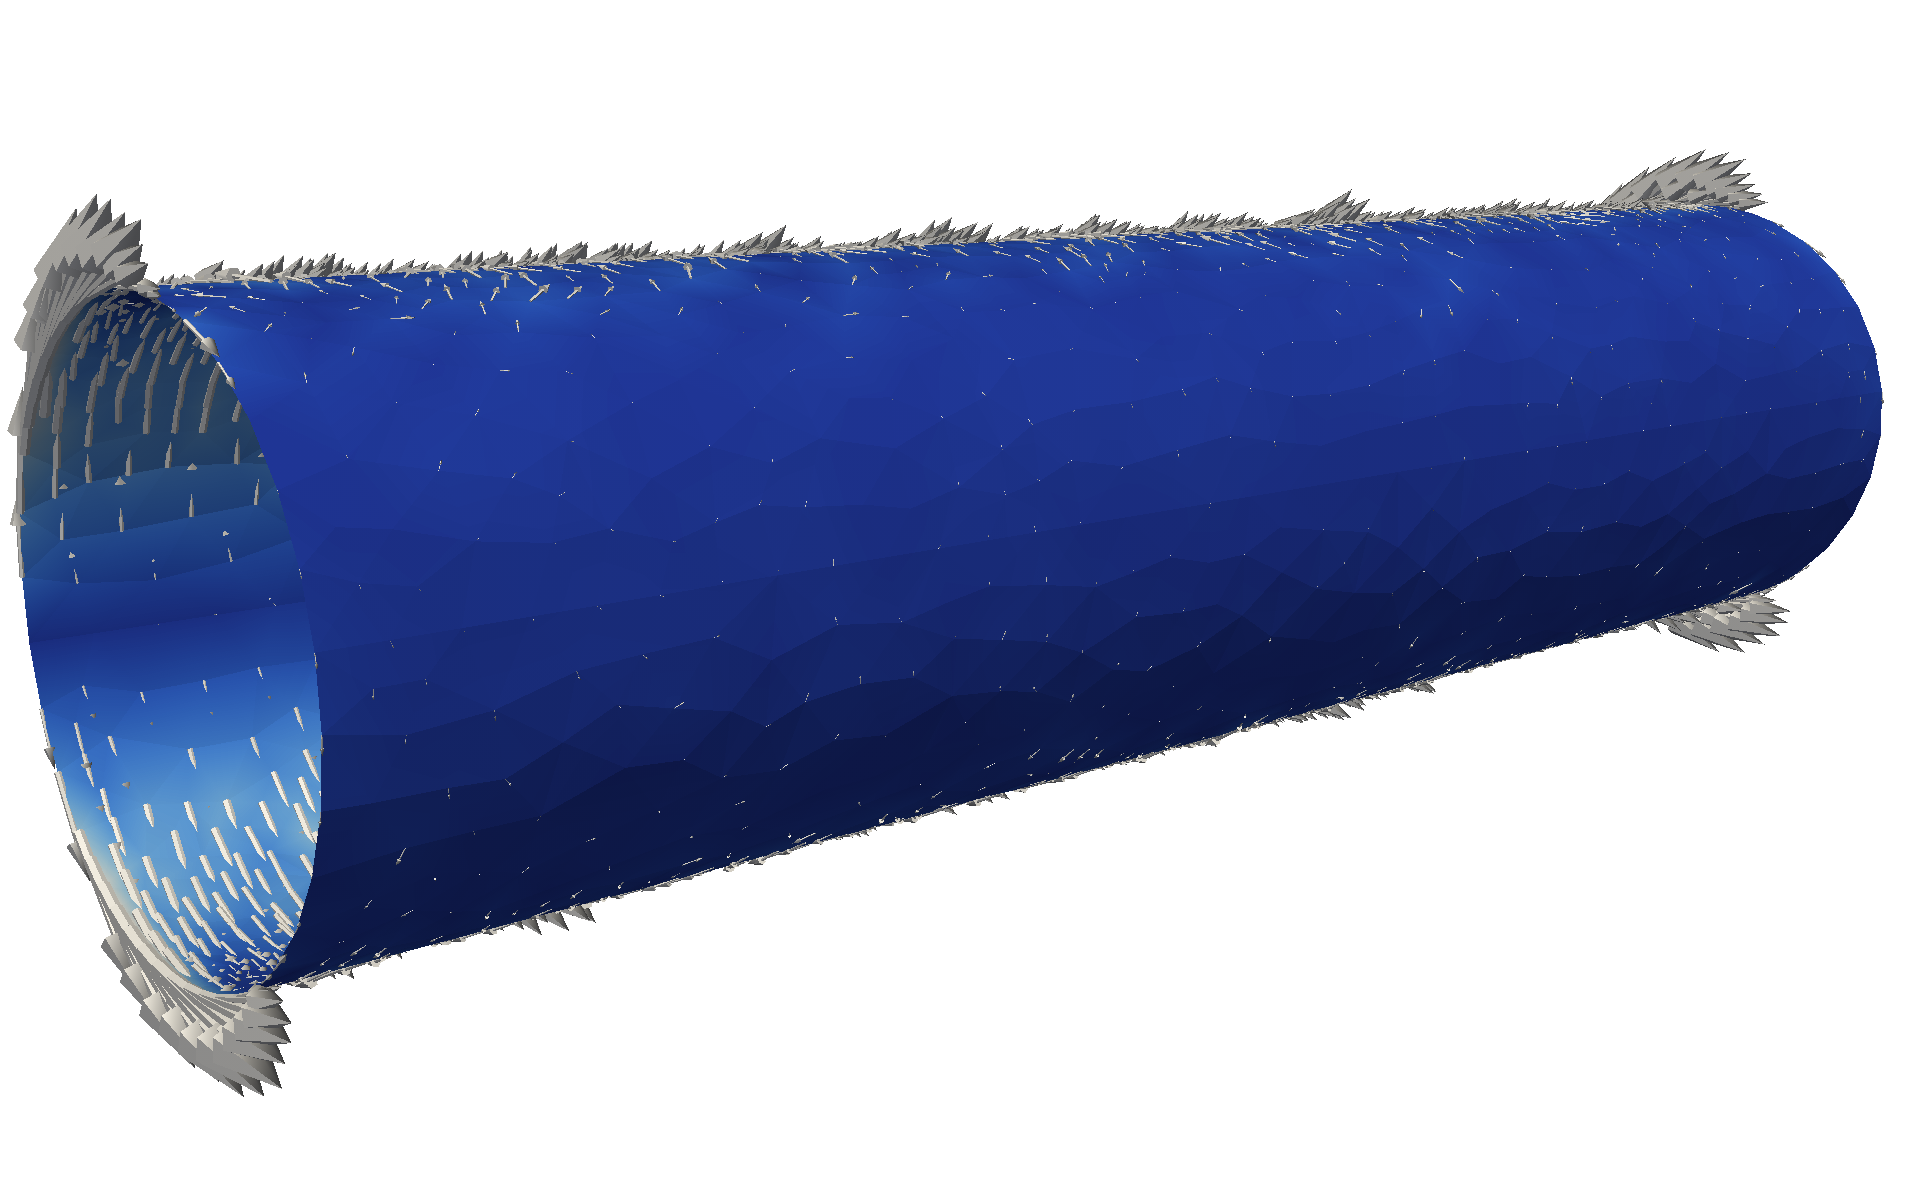
\includegraphics[height=4cm]{chapters/hoffman-1/png/Hoffman_fig2a.png}
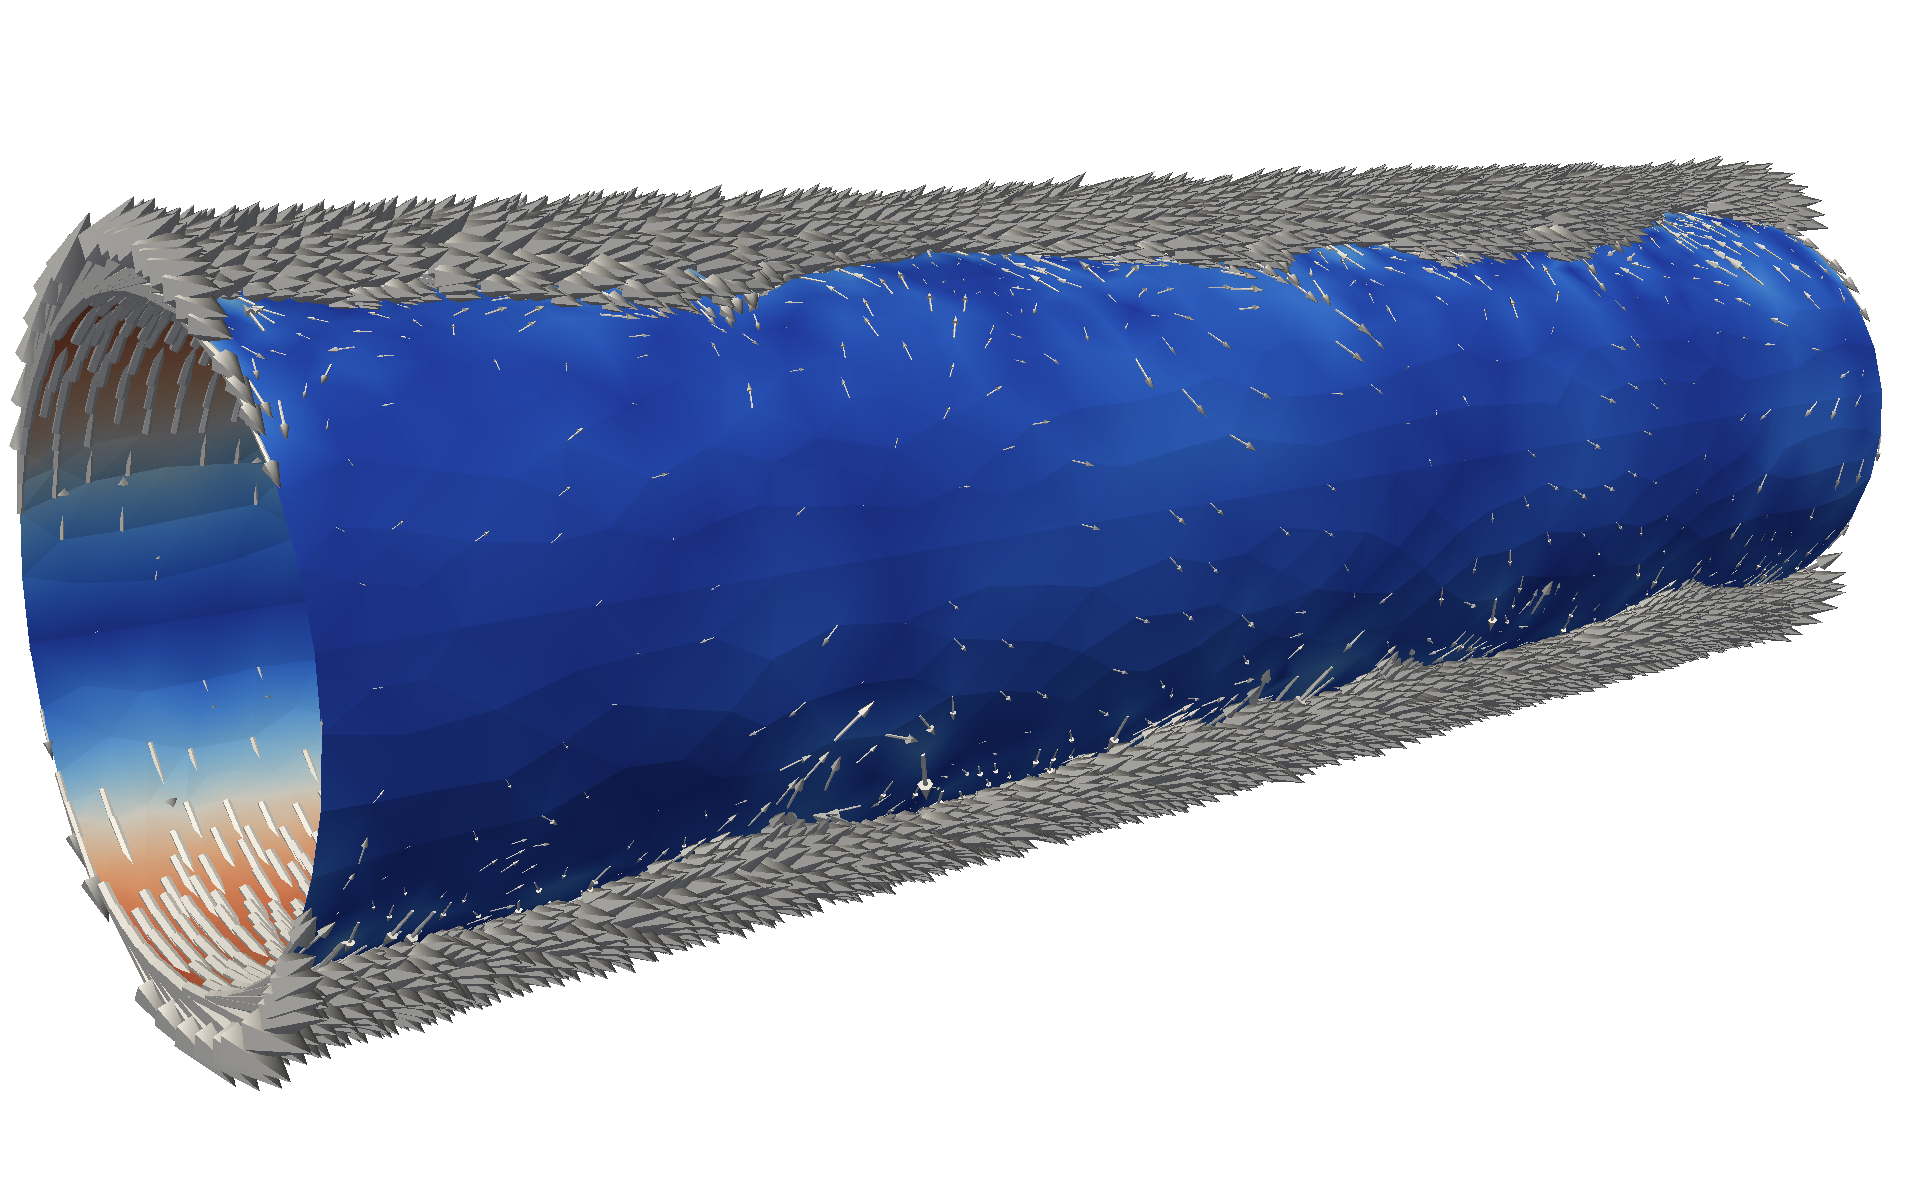
\includegraphics[height=4cm]{chapters/hoffman-1/png/Hoffman_fig2b.png}
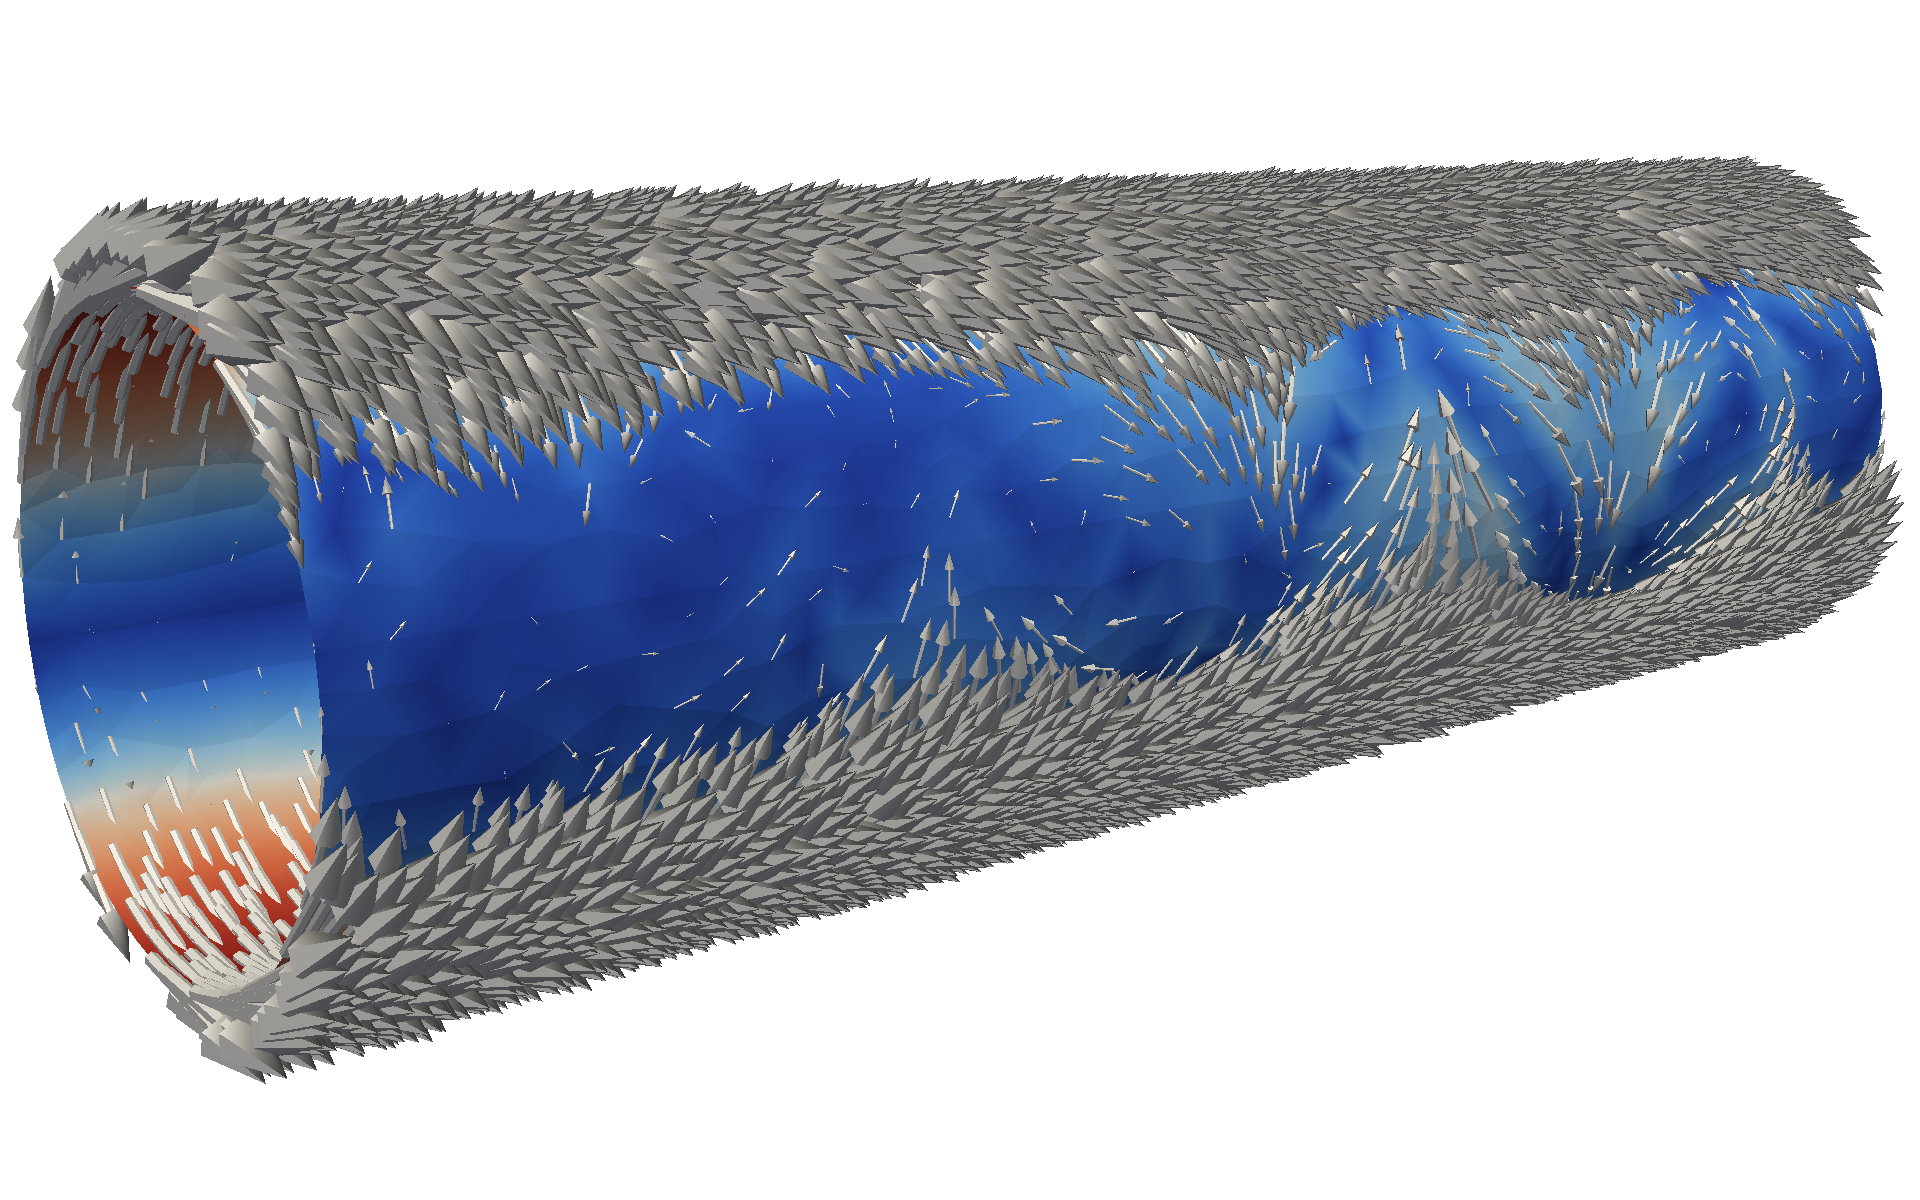
\includegraphics[height=4cm]{chapters/hoffman-1/png/Hoffman_fig2c.png}
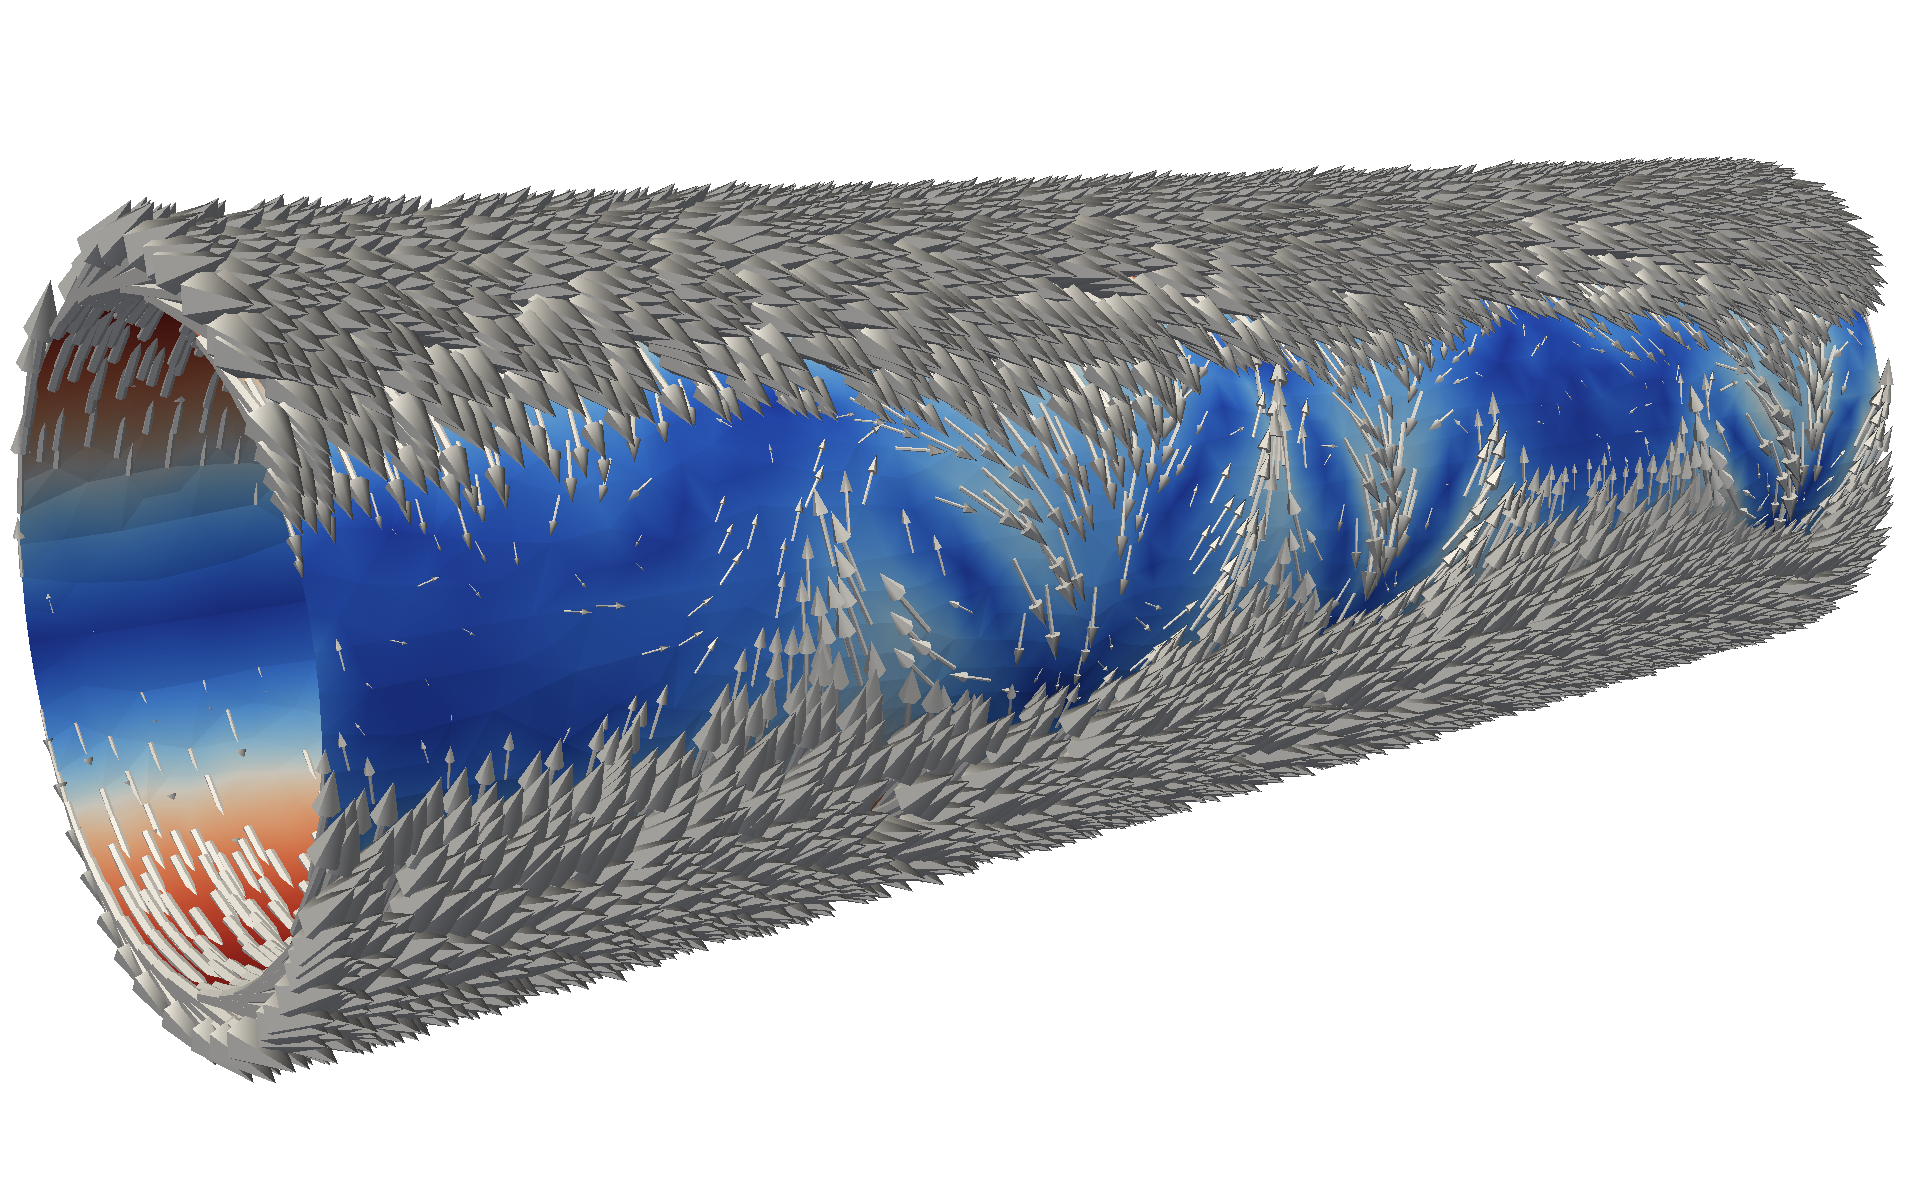
\includegraphics[height=4cm]{chapters/hoffman-1/png/Hoffman_fig2d.png}
\caption{Turbulent flow separation  \cite{HoffmanJansson2009}: velocity vectors at surface of cylinder; for $\beta = 10^{-1}$, $\beta = 10^{-2}$, $\beta = 10^{-3}$ and $\beta = 0$ (from upper left to bottom right).}
\label{fig:1}
\end{figure}

\begin{figure}
\centering
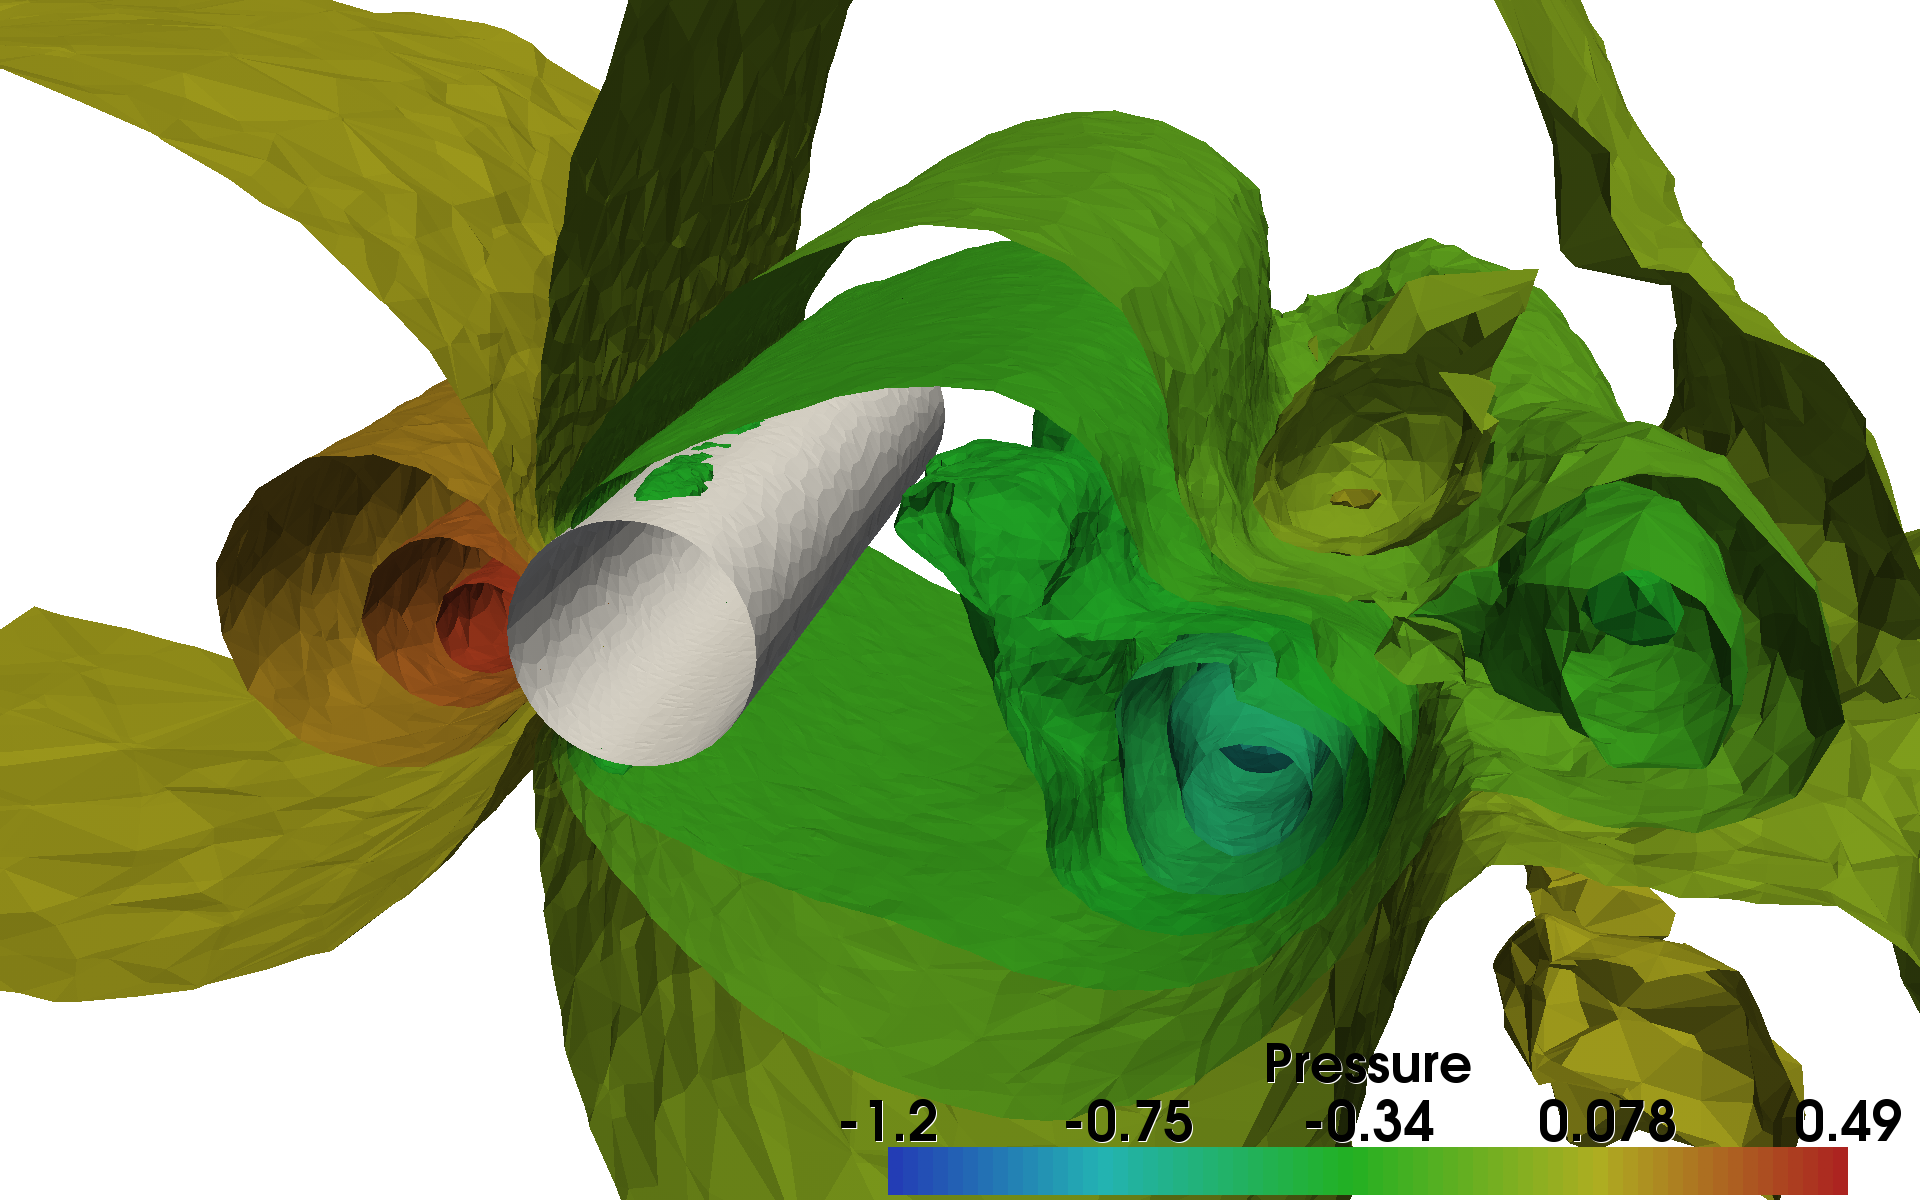
\includegraphics[height=4cm]{chapters/hoffman-1/png/Hoffman_fig3a.png}
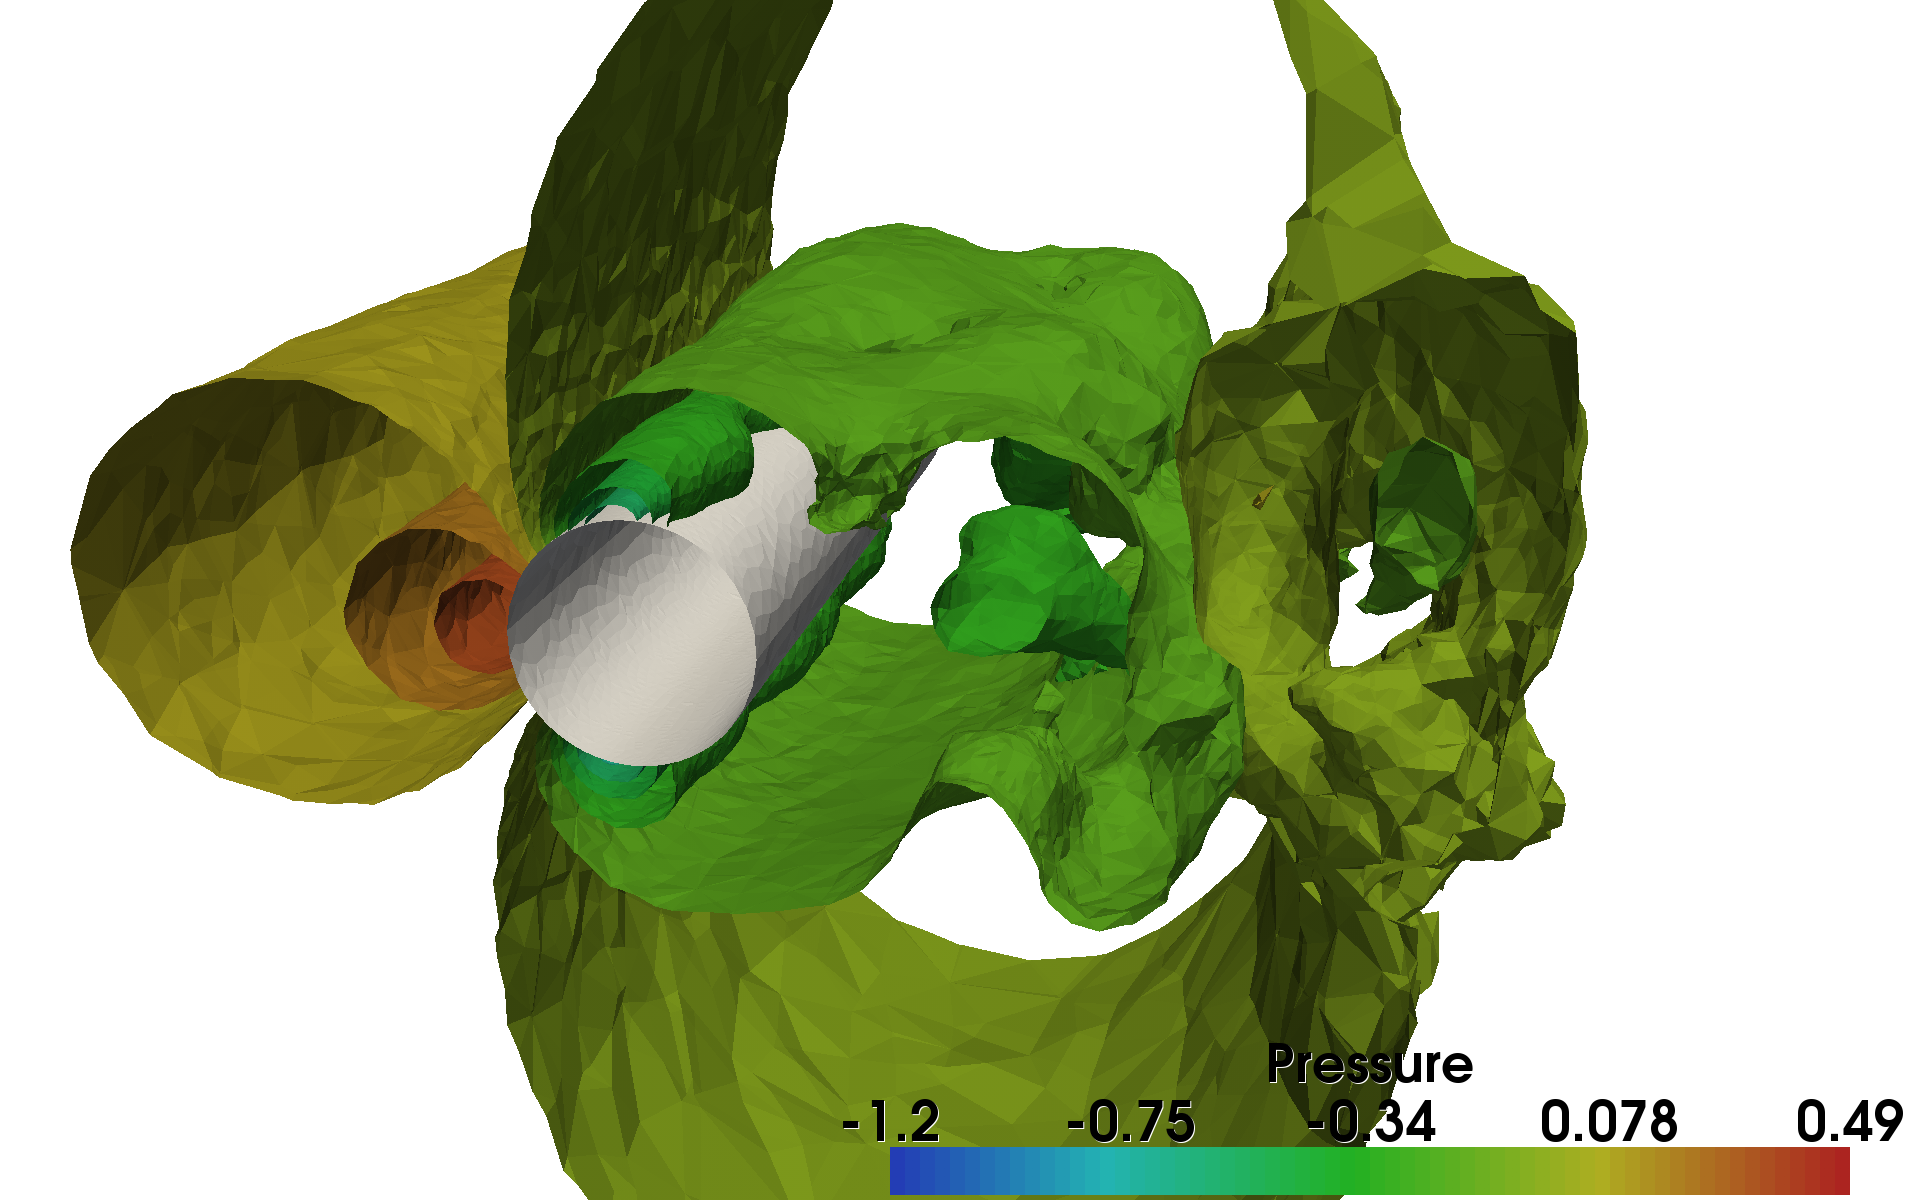
\includegraphics[height=4cm]{chapters/hoffman-1/png/Hoffman_fig3b.png}
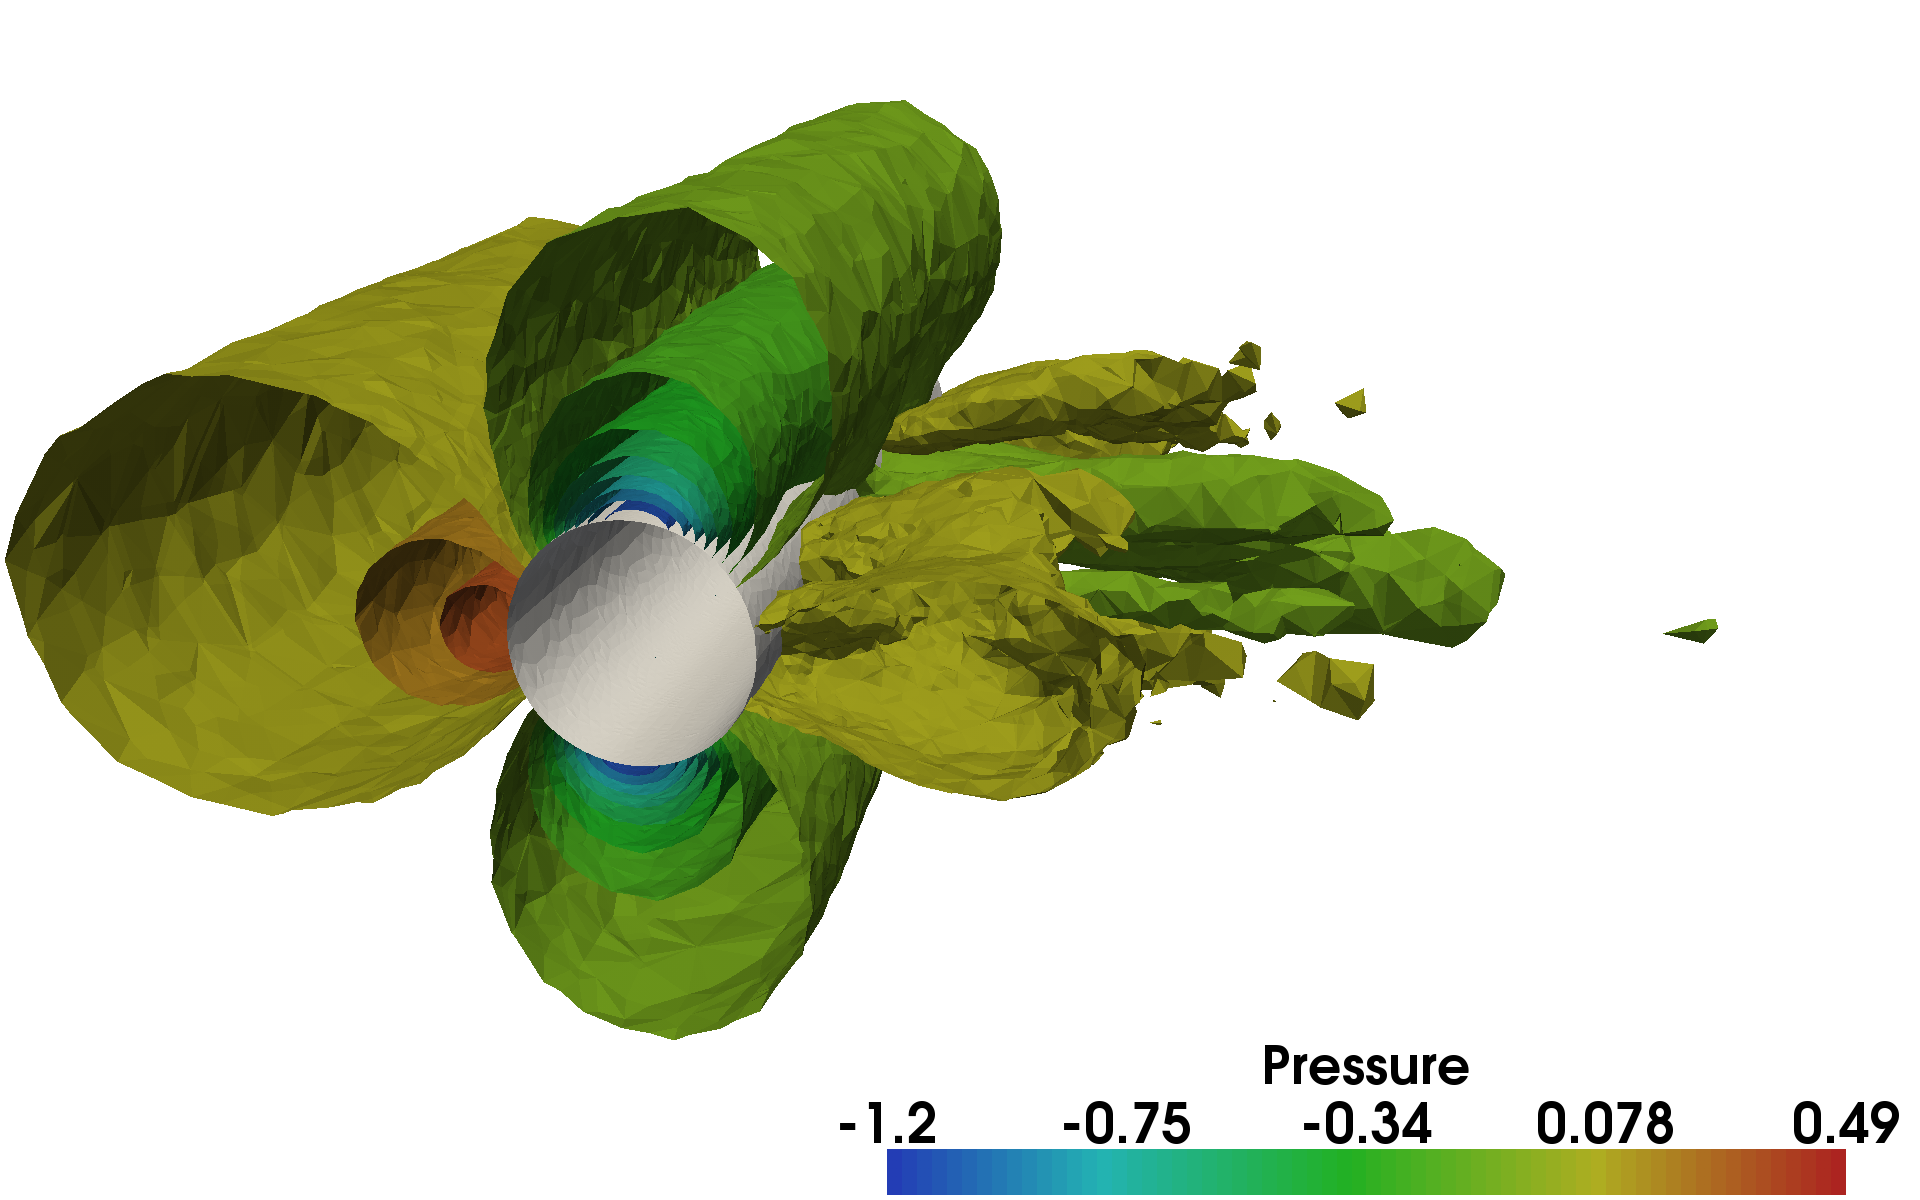
\includegraphics[height=4cm]{chapters/hoffman-1/png/Hoffman_fig3c.png}
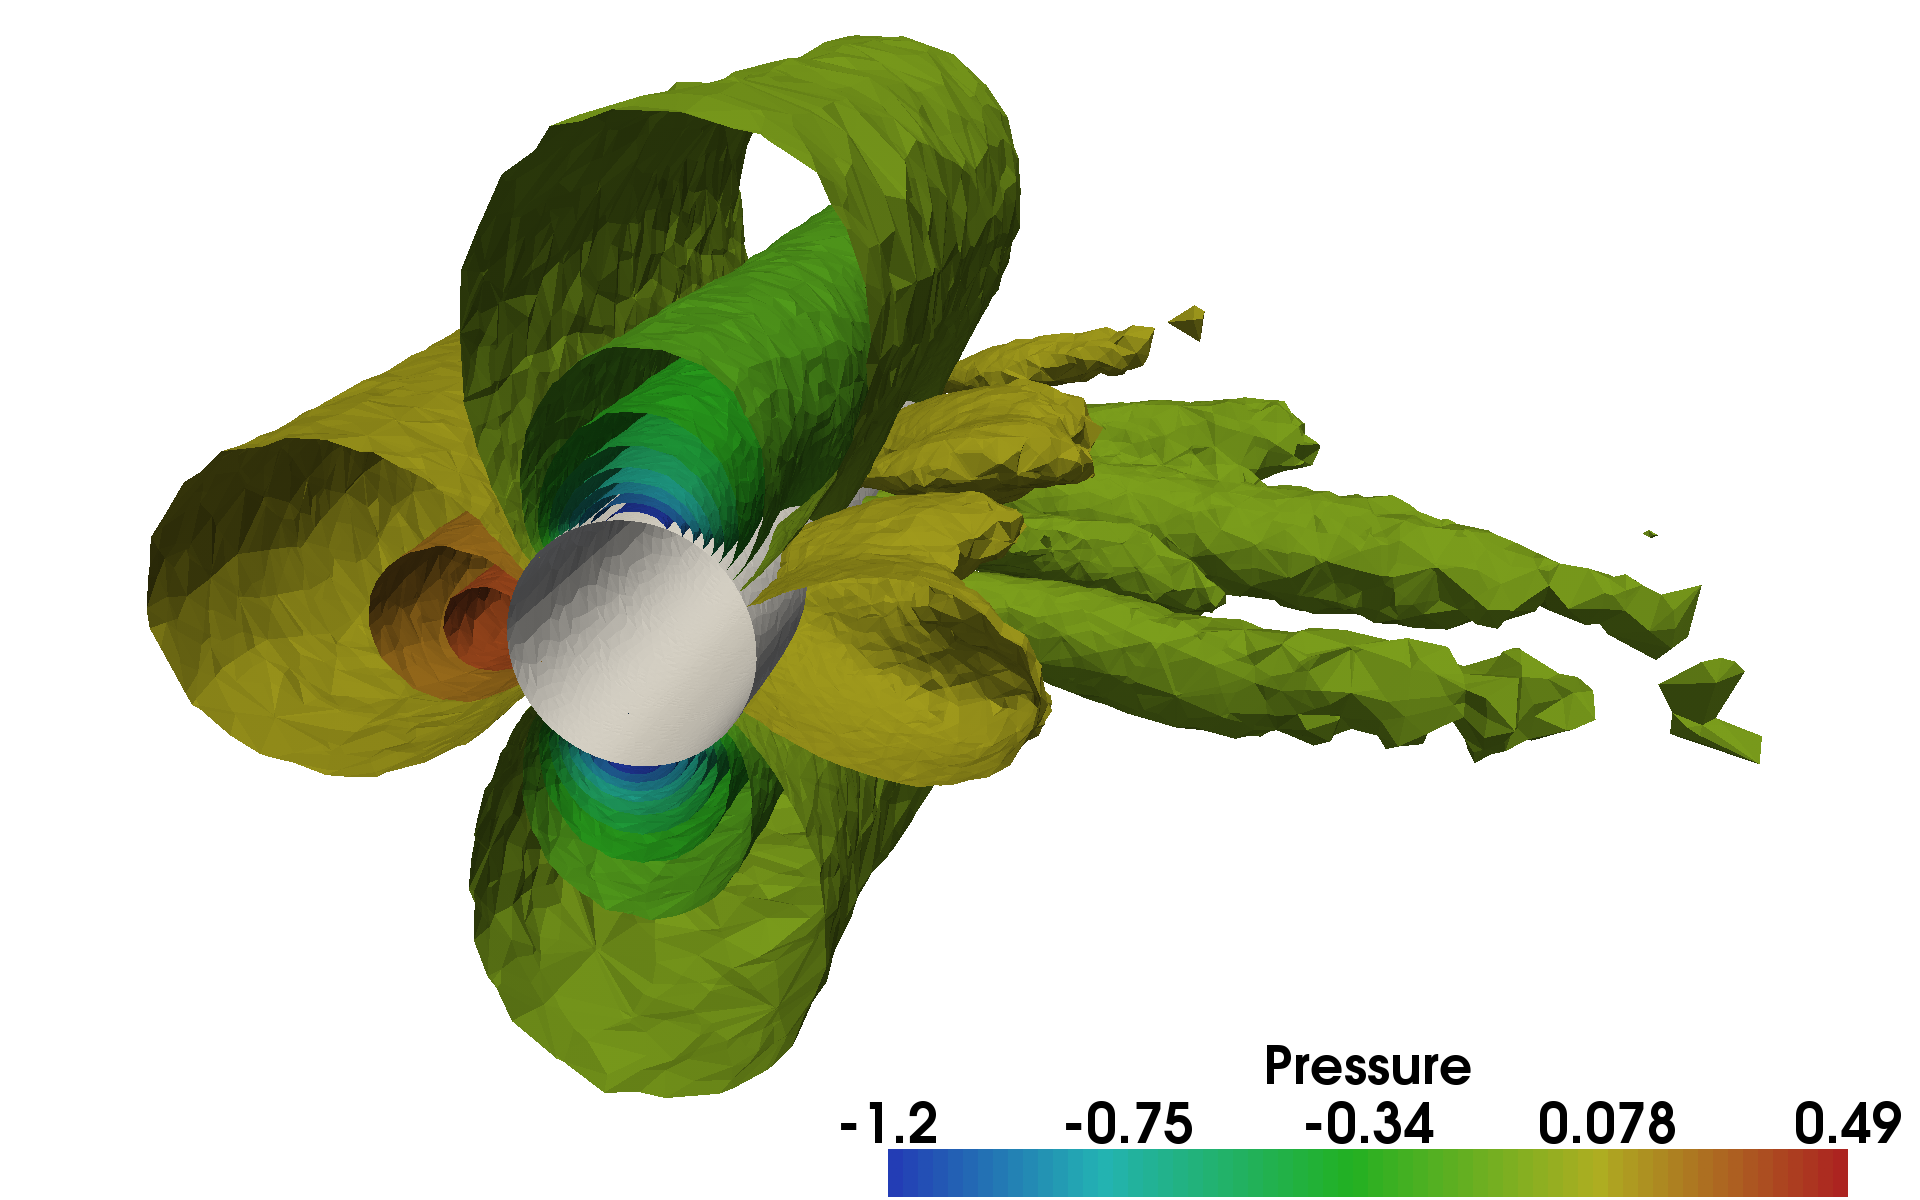
\includegraphics[height=4cm]{chapters/hoffman-1/png/Hoffman_fig3d.png}
\caption{Turbulent flow separation \cite{HoffmanJansson2009}: pressure isosurfaces; for $\beta = 10^{-1}$, $\beta = 10^{-2}$, $\beta = 10^{-3}$ and $\beta = 0$ (from upper left to bottom right).}
\label{fig:2}
\end{figure}

\begin{figure}
\centering
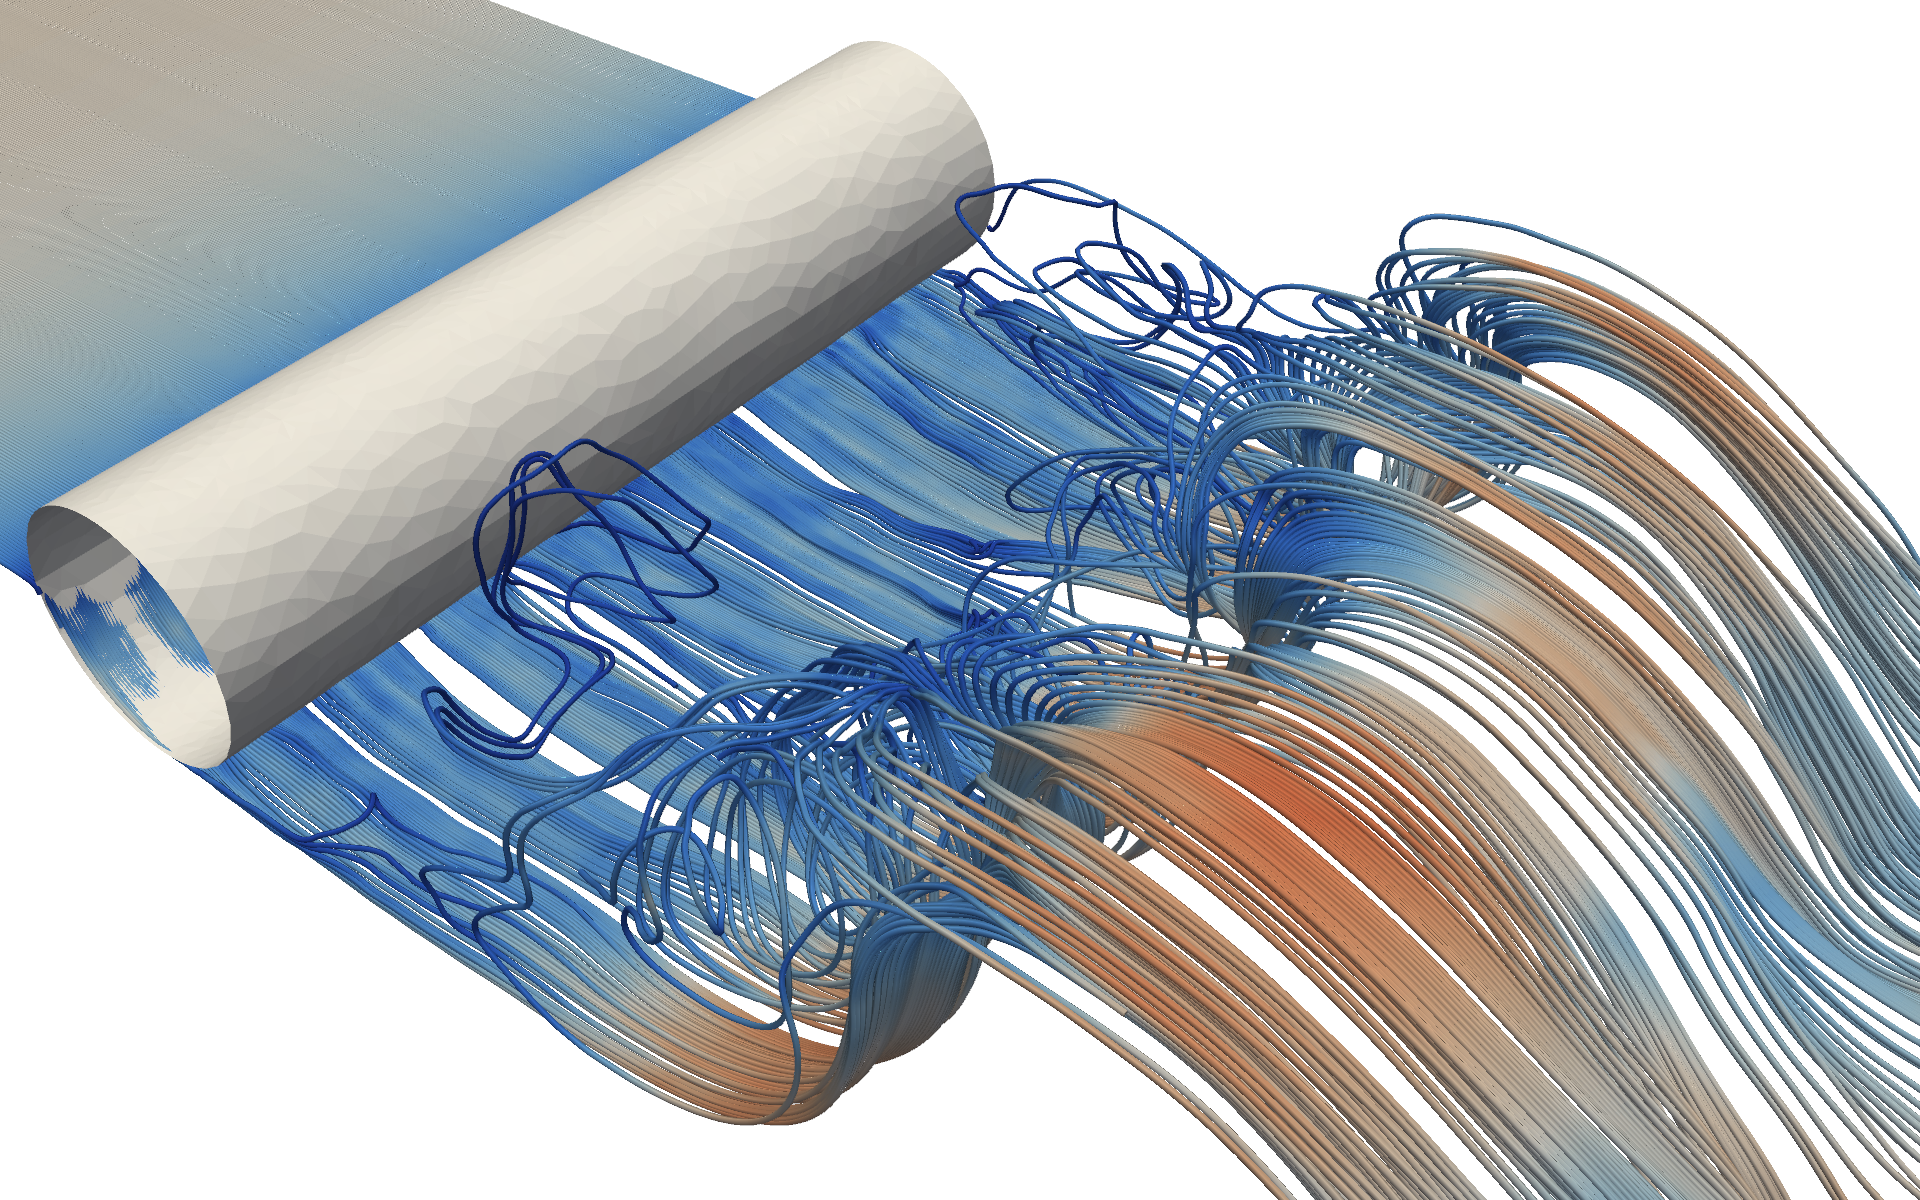
\includegraphics[height=4cm]{chapters/hoffman-1/png/Hoffman_fig5a.png}
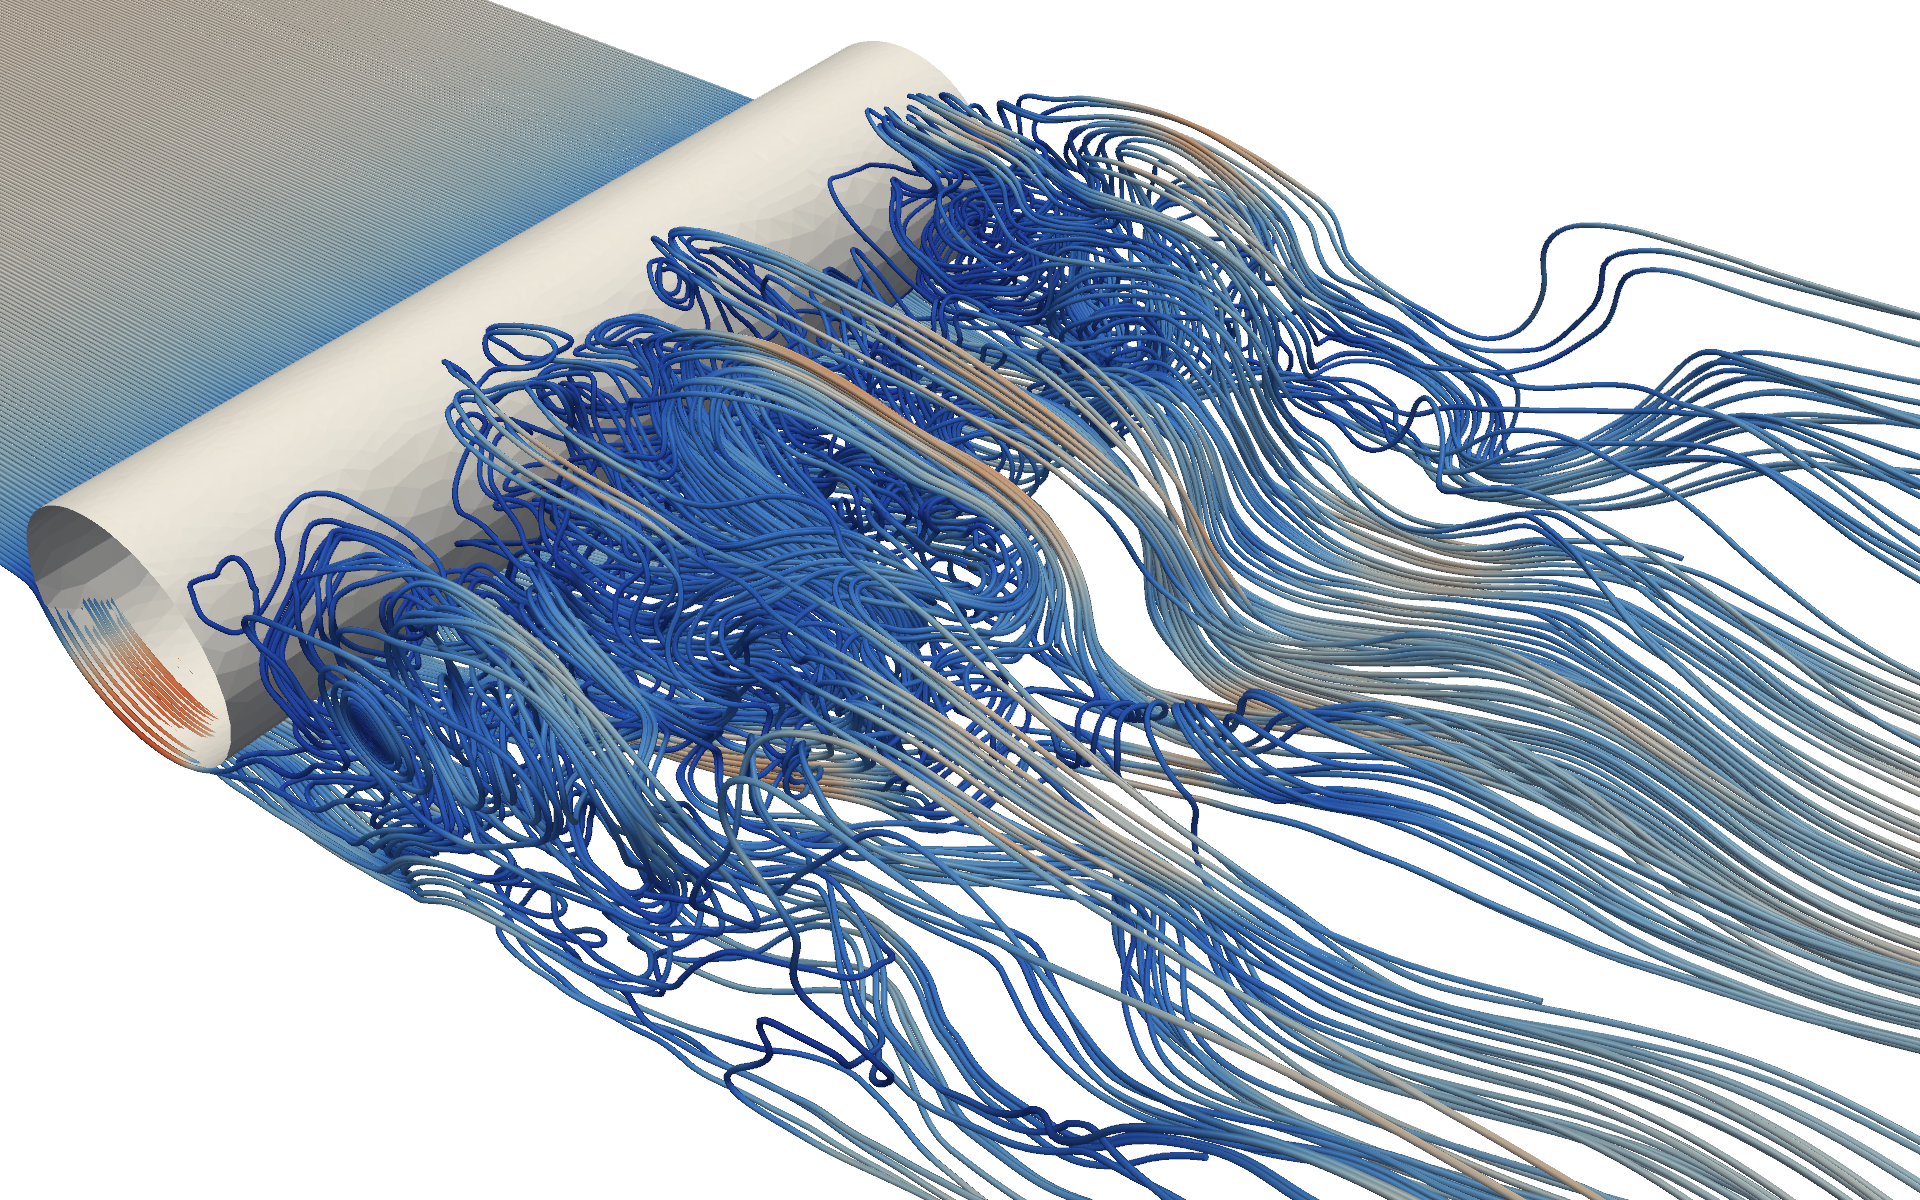
\includegraphics[height=4cm]{chapters/hoffman-1/png/Hoffman_fig5b.png}
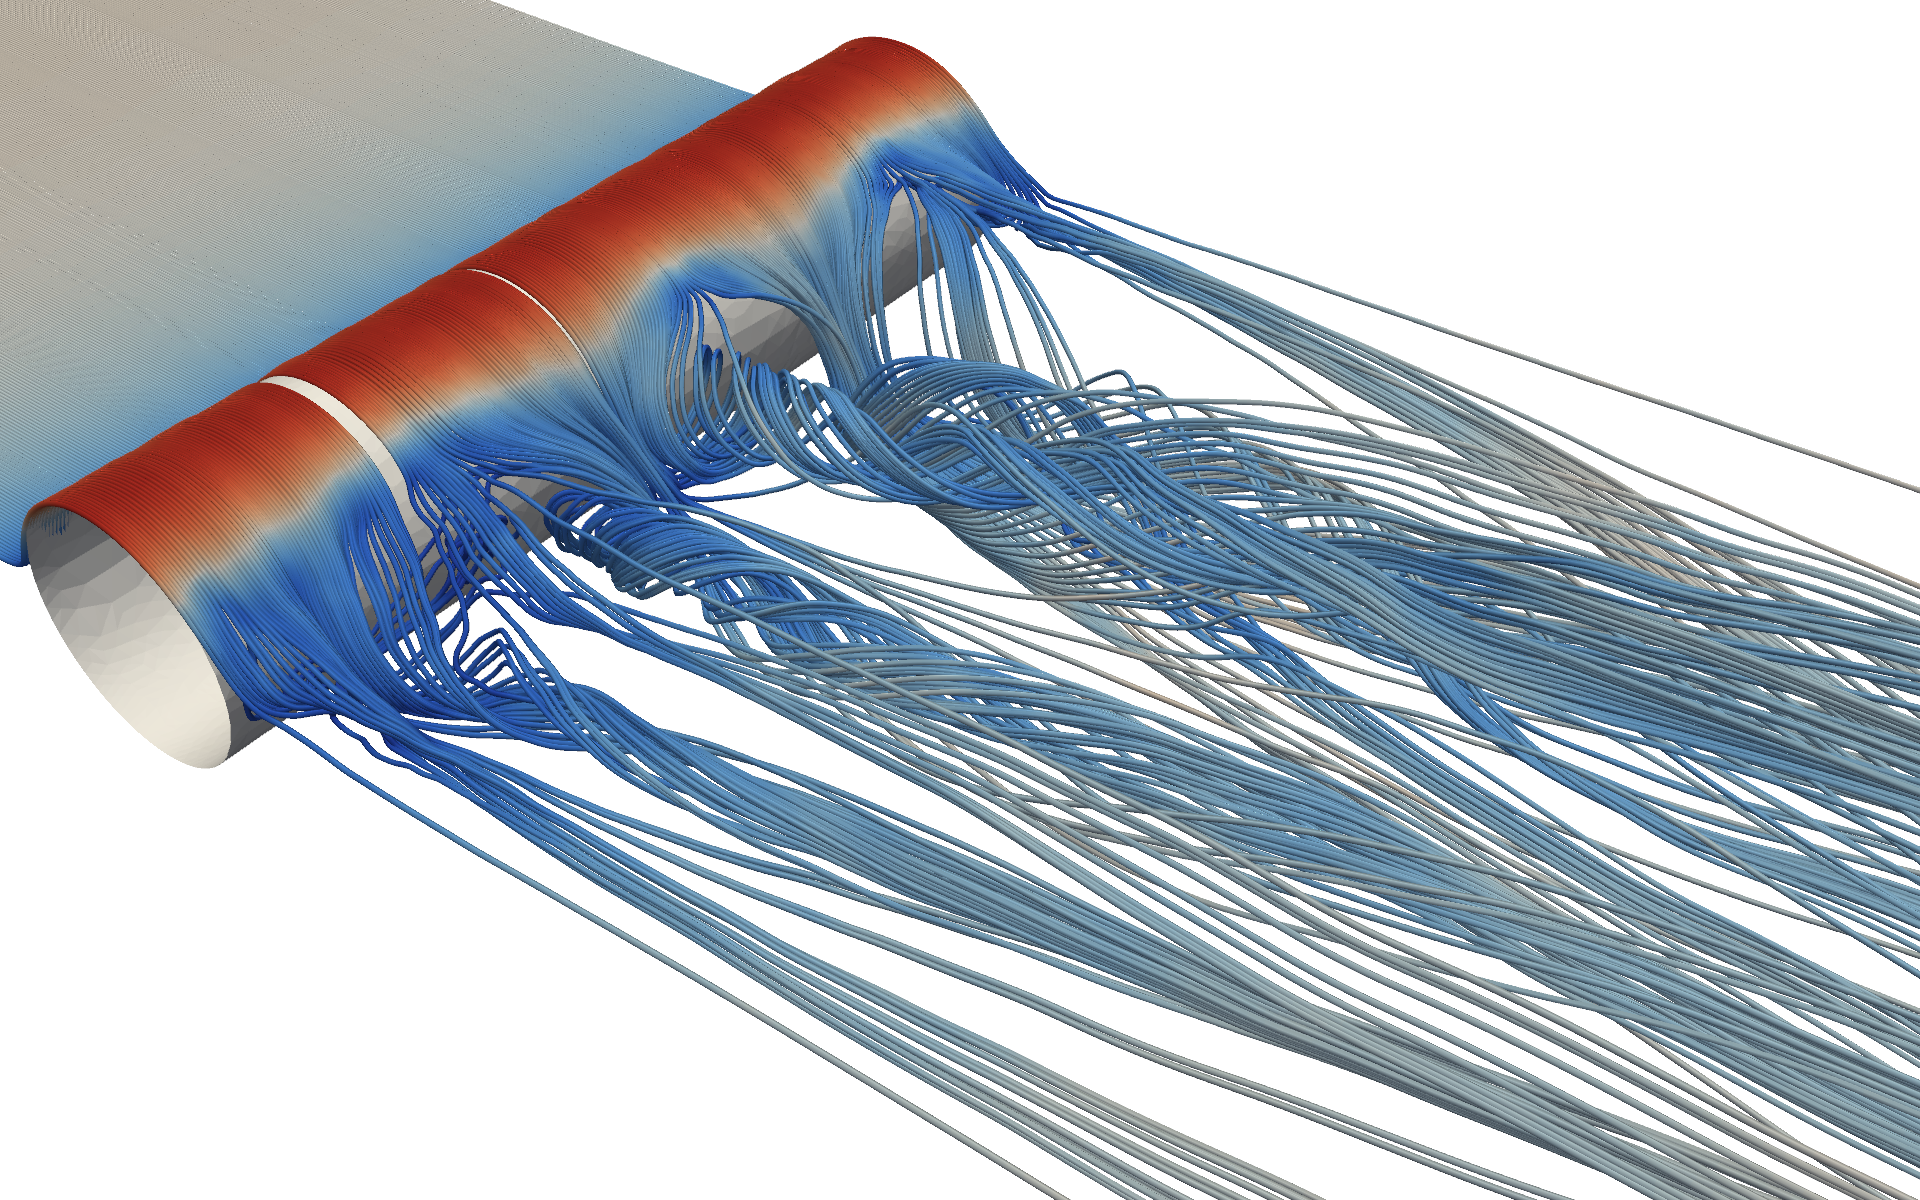
\includegraphics[height=4cm]{chapters/hoffman-1/png/Hoffman_fig5c.png}
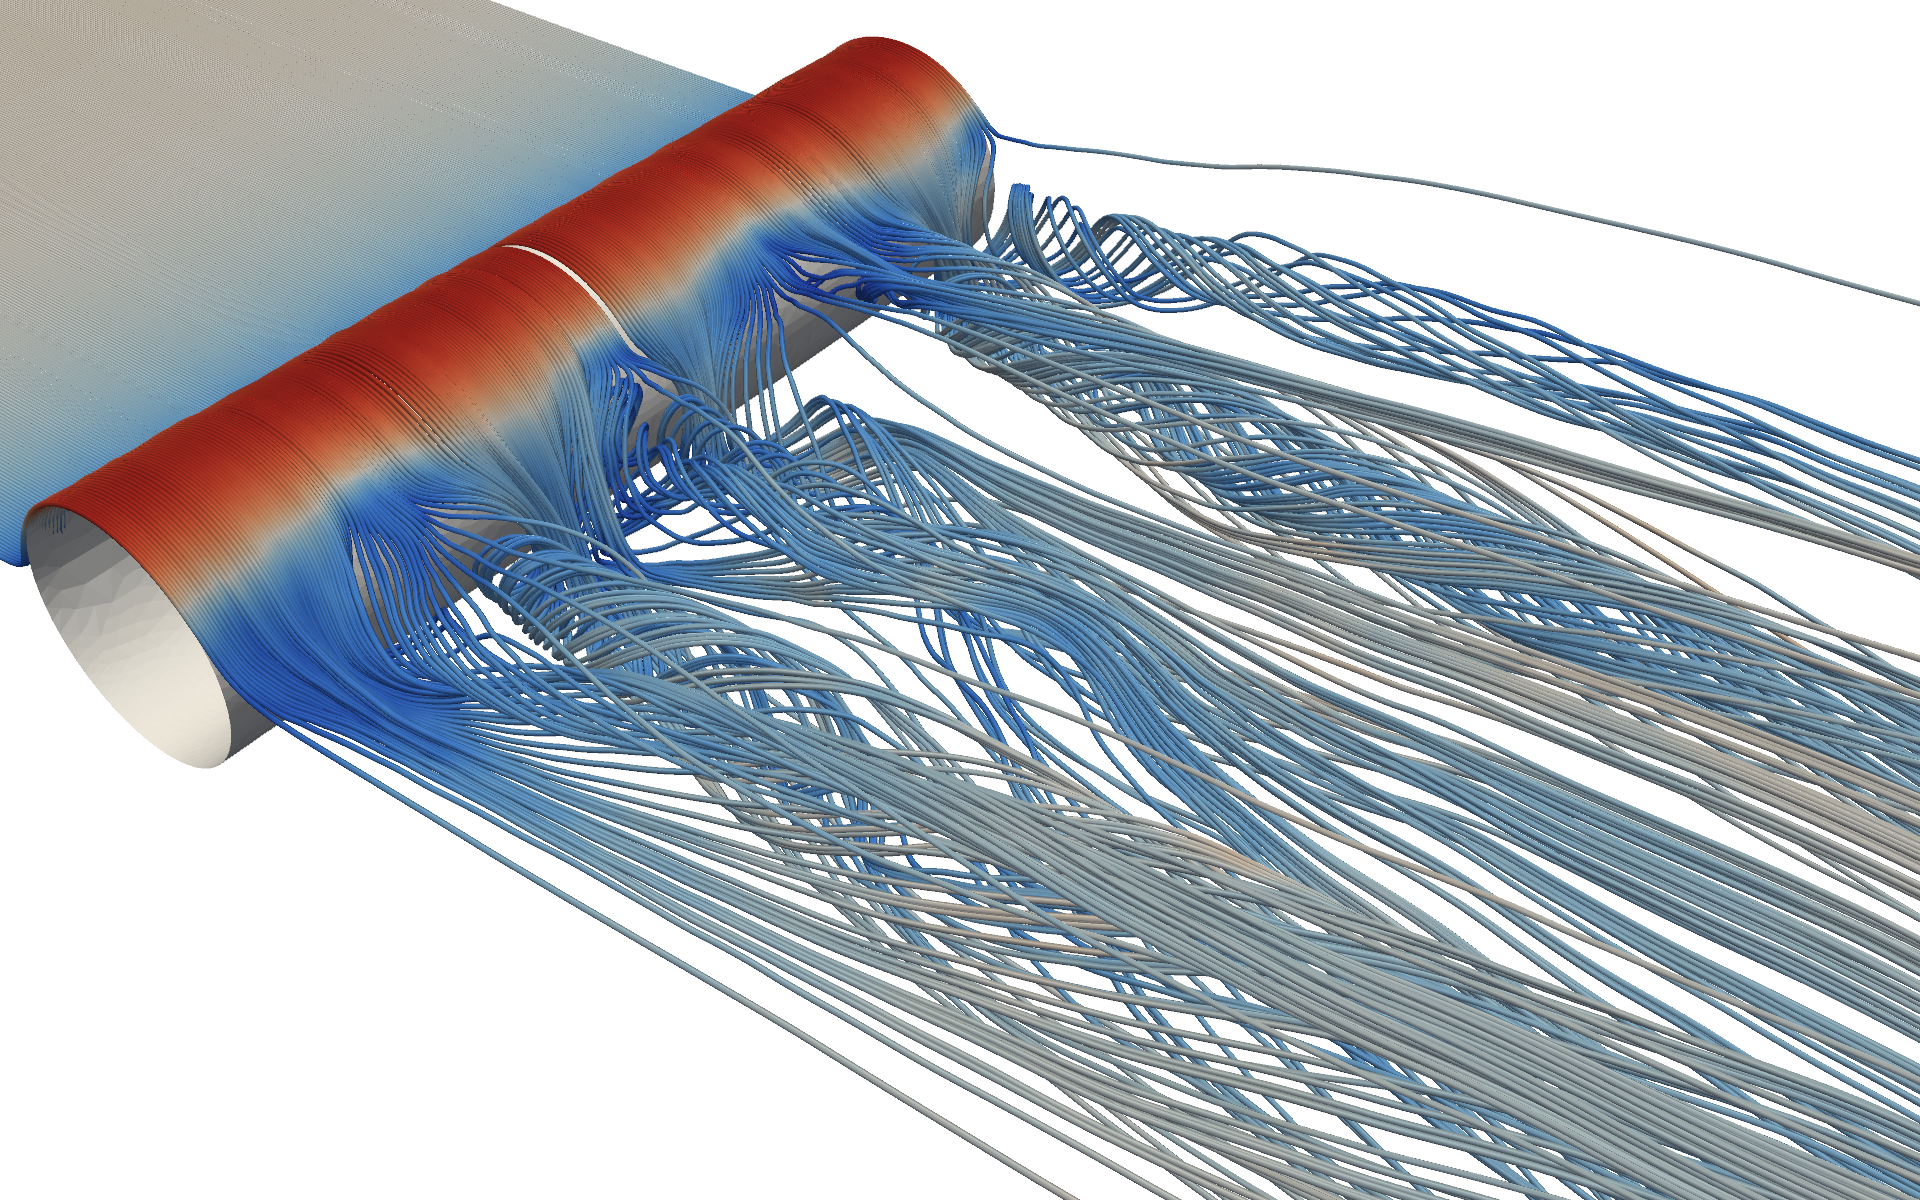
\includegraphics[height=4cm]{chapters/hoffman-1/png/Hoffman_fig5d.png}
\caption{Turbulent flow separation \cite{HoffmanJansson2009}: velocity streamlines; for $\beta = 10^{-1}$, $\beta = 10^{-2}$, $\beta = 10^{-3}$ and $\beta = 0$ (from upper left to bottom right).}
\label{fig:3}
\end{figure}

\subsection{Turbulent flow past complex geometry}

With the parallel implementation of Unicorn, realistic problems of complex geometry and high Re turbulent flow can be addressed. As an example, we present simulation results from the NASA/AIAA workshop "Benchmark problems for Airframe Noise Computations" (BANC-1), held in conjunction with the 16$^{th}$ AIAA/CEAS Aeroacoustics Conference in Stockholm in 2010, where Unicorn was used for adaptive simulation of flow past a rudimentary landing gear configuration \cite{VilelaJanssonEtAl2010}. The landing gear configuration was designed by Boeing, and detailed experimental results were available, as well as internal comparison within the participating groups \cite{SpalartMejia2011}.

Starting from a coarse mesh of ca 70,000 mesh points, the mesh was adaptively refined 7 times with respect to the error in the drag force on the landing gear. The resulting final mesh had 1,000,000 mesh points, and the computation ran on the \textit{Akka} computer at HPC2N using 264 number of cores. The skin friction boundary layer model was used with $\beta=0$, thus corresponding to a slip boundary condition.

The Unicorn contribution to the workshop compared well with other participating groups, with overall little spread in the computation of aerodynamic forces, and mean sound pressure levels. Also mean flow patterns on the surface of the landing gear (see Fig.\ref{rlg}) showed good agreement with experimental results. Other quantities, such as frequencies, showed a wide spread among the participating groups, and cannot serve as a benchmark test of Unicorn in this setting.

Thanks to the adaptive mesh refinement and the cheap boundary layer model, the Unicorn results were obtained with very few mesh points, less than all other participating groups in the workshop, see Table \ref{tab:hoffman-1-rlg}.

\begin{figure}
\centering
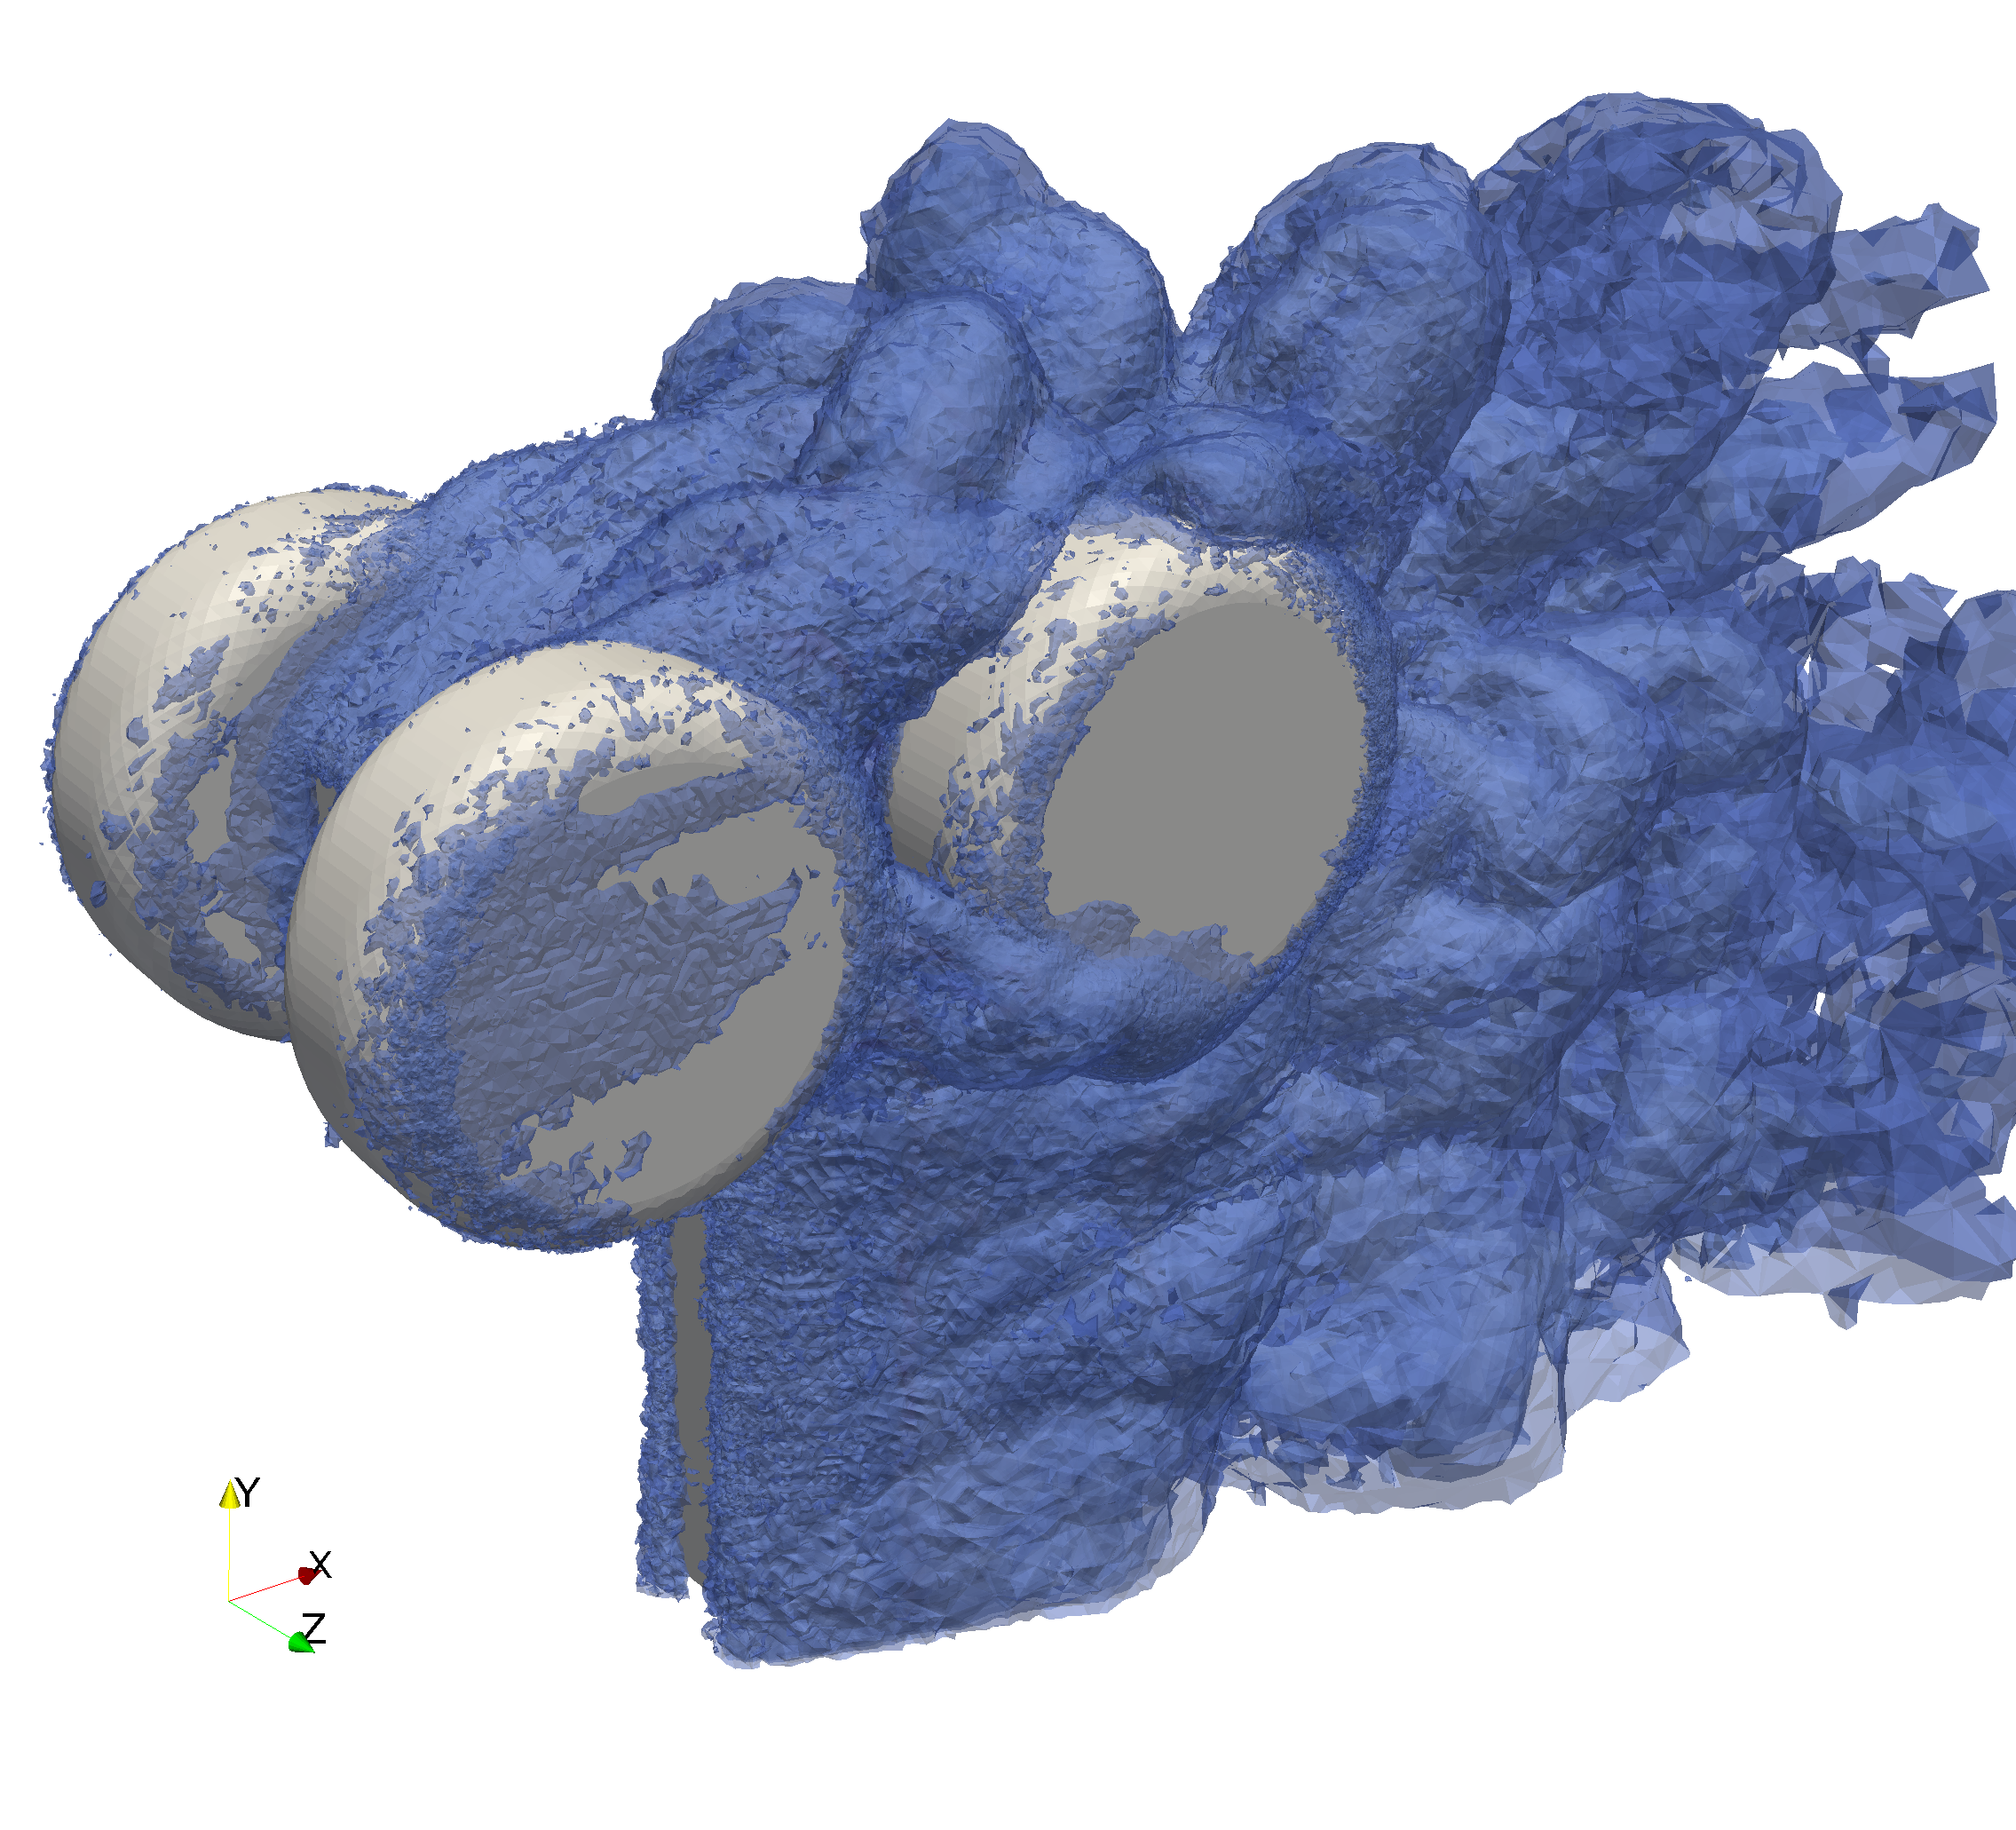
\includegraphics[height=6cm]{chapters/hoffman-1/png/rlg_vorticity}
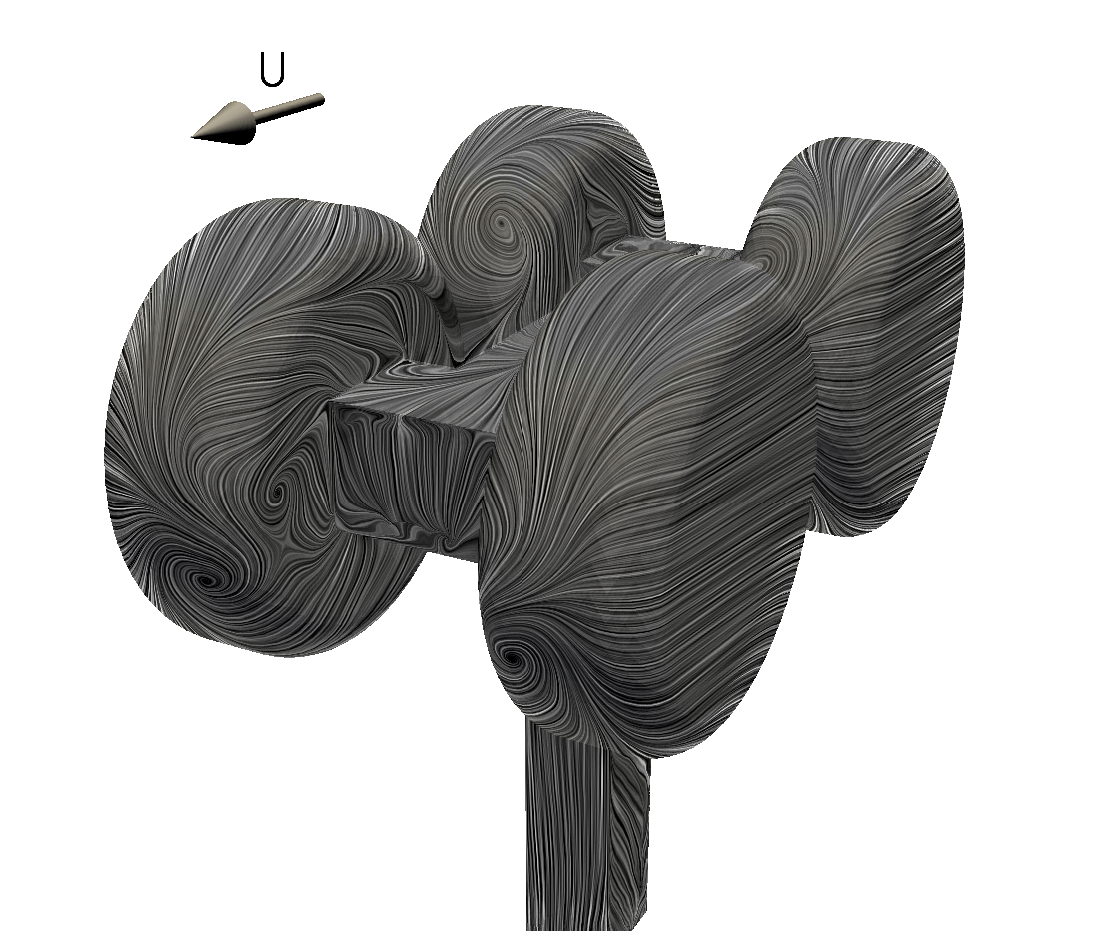
\includegraphics[height=6cm]{chapters/hoffman-1/png/oilfilm_back_sim}
\caption{Rudimentary landing gear: plot of simulated vorticity (upper) and simulated oil film patterns (lower).}
\label{rlg}
\end{figure}

\begin{table}[hbt]
\begin{center}
\begin{tabular}{|c|cc|}
\hline
Team & $C_D$ & \#Cells \\
\hline
NTS &    1.70 &    10M \\
CDA  &   1.70  &   29M \\
\textbf{KTH}  &   \textbf{1.78}  &   \textbf{6M}\\
KHI  &   1.81  &   41M \\
EXA  &   1.77  &   36M \\
TUB  &   1.74  &   11M \\
\hline
\end{tabular}
\caption{\label{tab:hoffman-1-rlg} Drag coefficient and number of cells for each of the teams in BANC-1 \cite{SpalartMejia2011}. The Unicorn results are the ones by the KTH-team.}
\end{center}
\end{table}

\subsection{Robust fluid--structure interaction}

As a quantitative test of the Unicorn FSI solver we consider the benchmark problem FLUSTRUK-A, variant 3, which is defined in \cite{HronTurek2005}. This is a 2D flow in a channel past a fixed cylinder with a thin flexible bar attached to the downstream side of the cylinder. The Unicorn results are compared to the reference results of 2 other groups: Hron/Turek \cite{HronTurek2005} and Dunne/Rannacher \cite{DunneRannacher2006}.

The y-displacement in the oscillation regime varies between 0.0353m and -0.0332m (see Fig.\ref{fig:flustruk}), which is within 1-2\% of the Hron/Turek results, and within 11\% of the Dunne/Rannacher amplitude. The oscillation frequency is estimated to 5.3Hz from the graph, where the Hron/Turek frequency is estimated to 5.4Hz and the Dunne/Rannacher frequency is given as 5.48 Hz. The Unicorn results are thus within 1-2\% of both groups. See \cite{HoffmanJanssonStockli2011} for a full discussion of the results, where also additional basic benchmark results are presented.

\begin{figure}[!h]
\center{
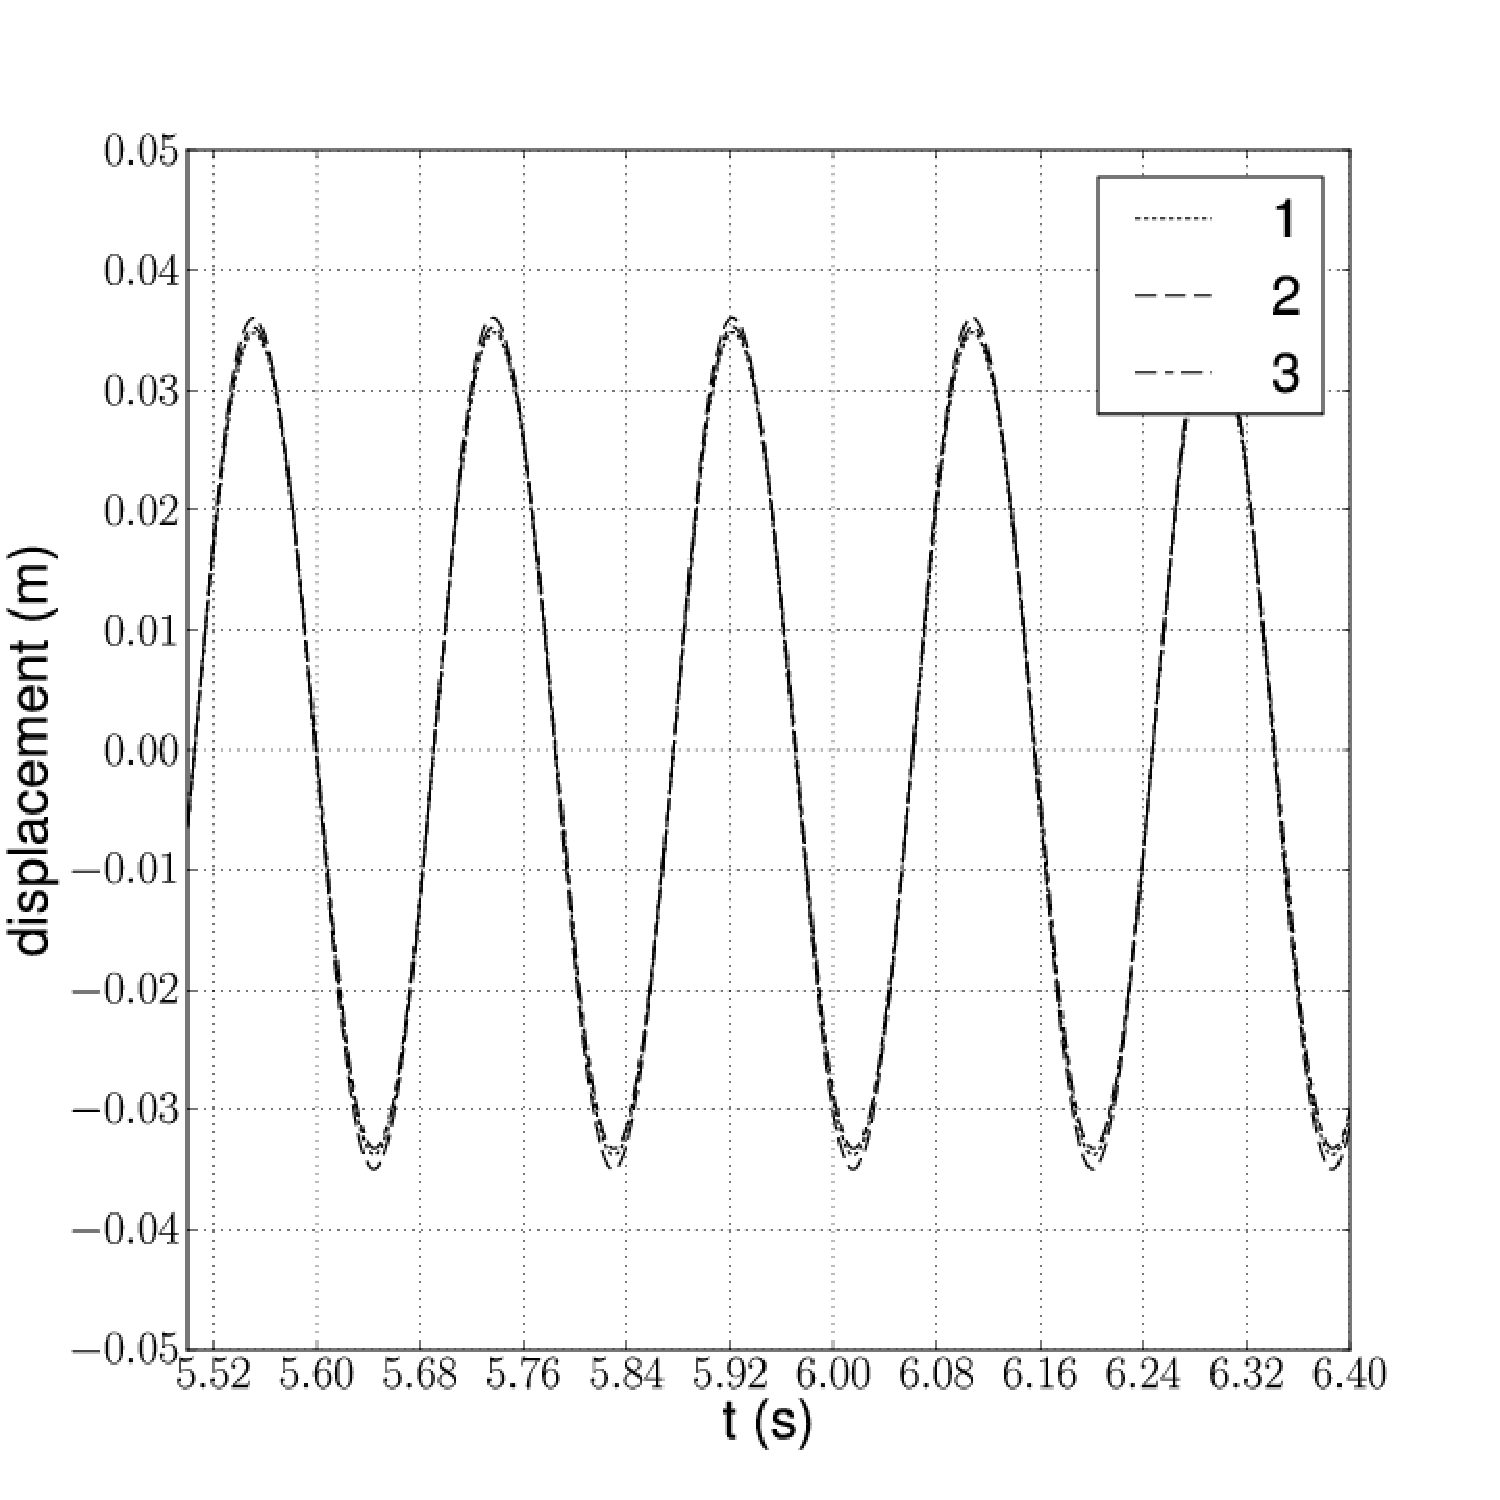
\includegraphics[width=10cm]{chapters/hoffman-1/png/fsi_bench3D_displacement_aligned.pdf}
}
\caption{
The figure shows the displacement along $y$-axis of the reference point in 2D FSI-benchmark problem FLUSTRUK-A  \cite{HoffmanJanssonStockli2011}, phase aligned to avoid start-up effects, for a sequence of three uniformly refined meshes using Unicorn.
}
\label{fig:flustruk}
\end{figure}

Unicorn target large structure deformations interacting with turbulent fluid flow. In Fig.\ref{fig:flag} we present qualitative results for a model problem of a flexible structure interacting
with turbulent flow in 3D, in the form of a fixed cube in turbulent flow with a thin flexible flag mounted in the downstream wake.

We choose an inflow speed of 1.0e2 m/s, a cube of 1.0e-2 m side and a flag mounted at the top of the back face of the cube with a length of 3.0e-1 m and a thickness of 5.0e-2 m. The viscosity of the fluid of 1.0e-4 Pa s (density $\rho=1$) which gives a representative Reynold's number $Re$ = 1.0e5. We choose no-slip boundary conditions on the cube and flag with slip boundary conditions on the surrounding channel walls, and a zero pressure outflow condition.

Violent bending and torsion motion along the long axis of the flag is observed, and we note that the
method is robust for these large structure deformations and highly fluctuating flow.

\begin{figure}[!h]
\center{
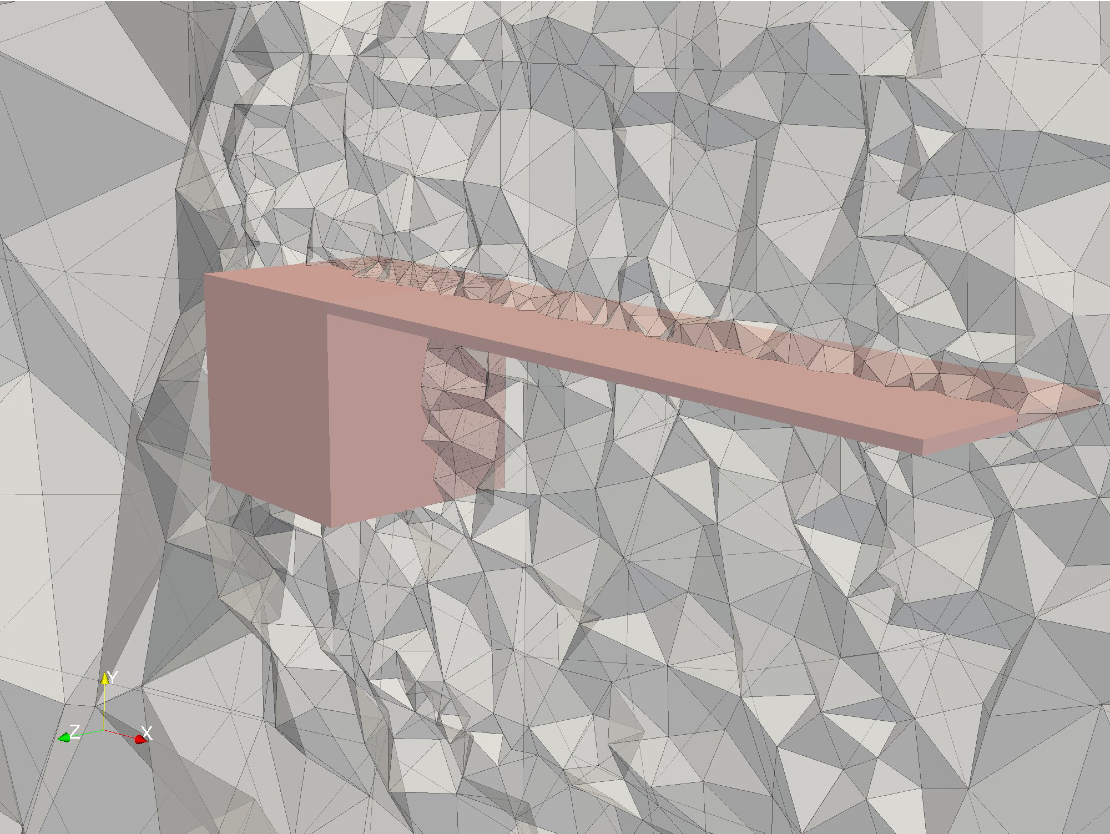
\includegraphics[width=5cm]{chapters/hoffman-1/png/cube000.png}
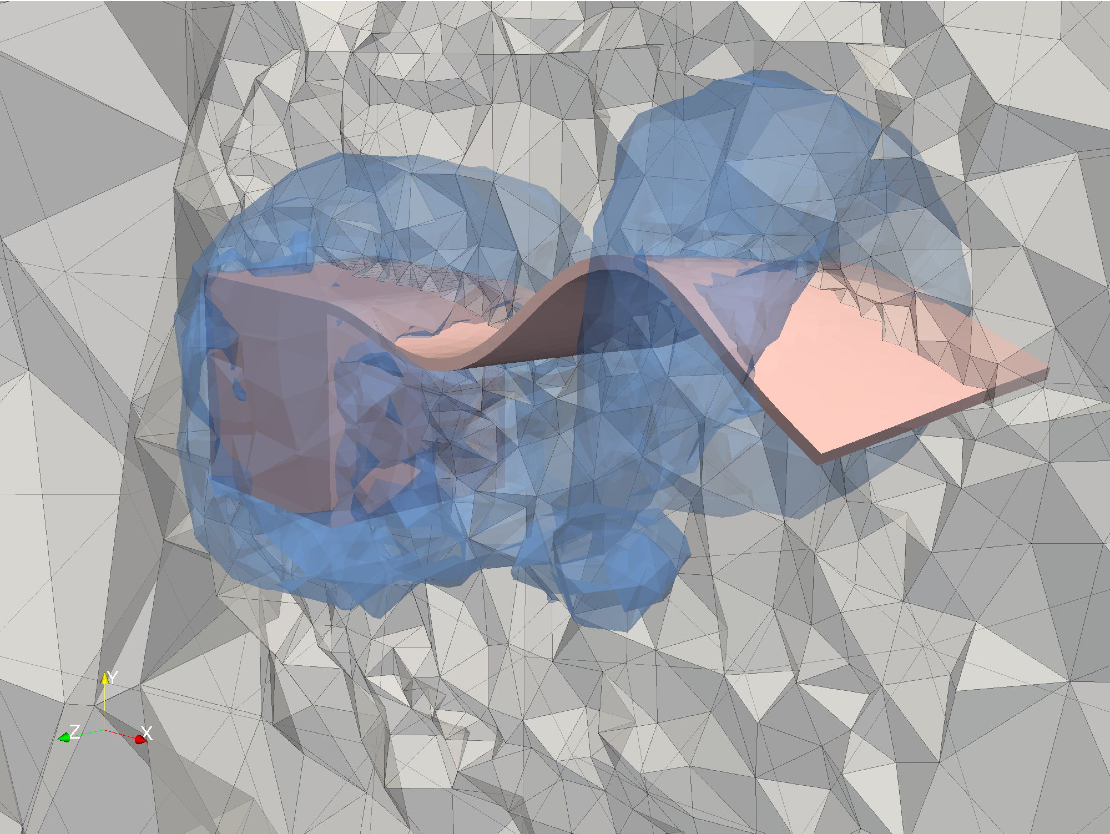
\includegraphics[width=5cm]{chapters/hoffman-1/png/cube115.png}\\
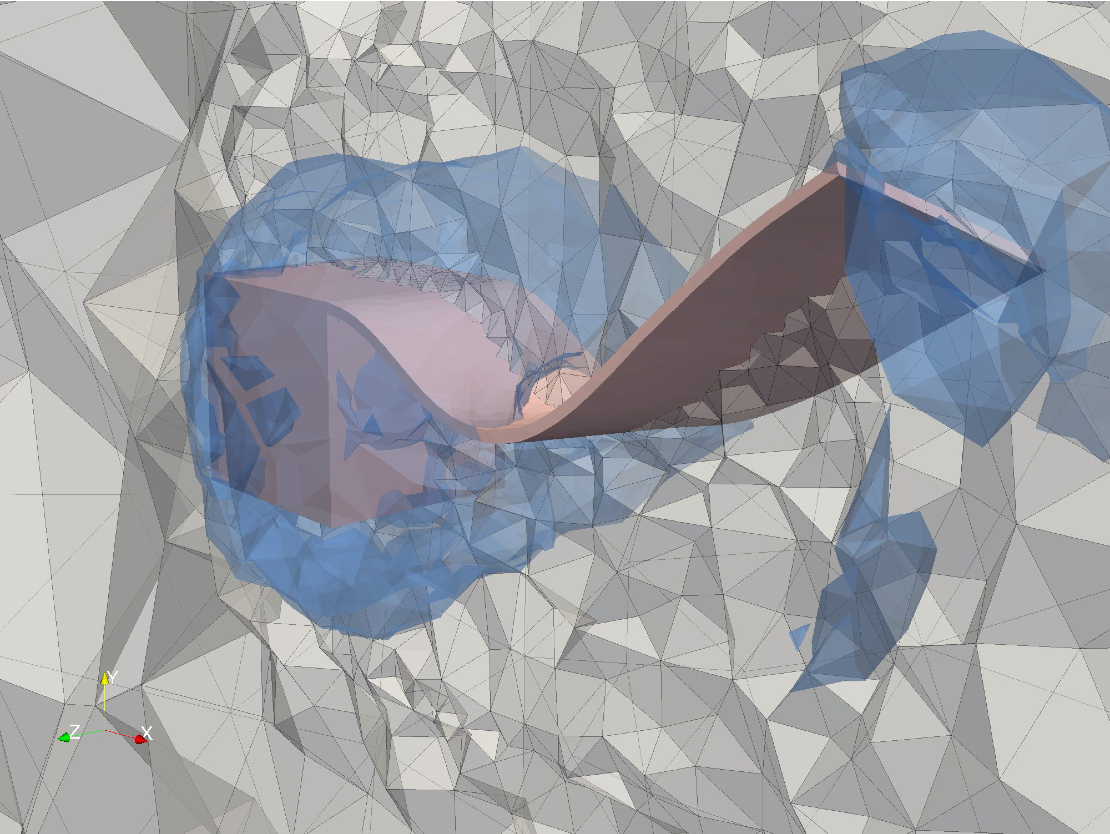
\includegraphics[width=5cm]{chapters/hoffman-1/png/cube125.png}
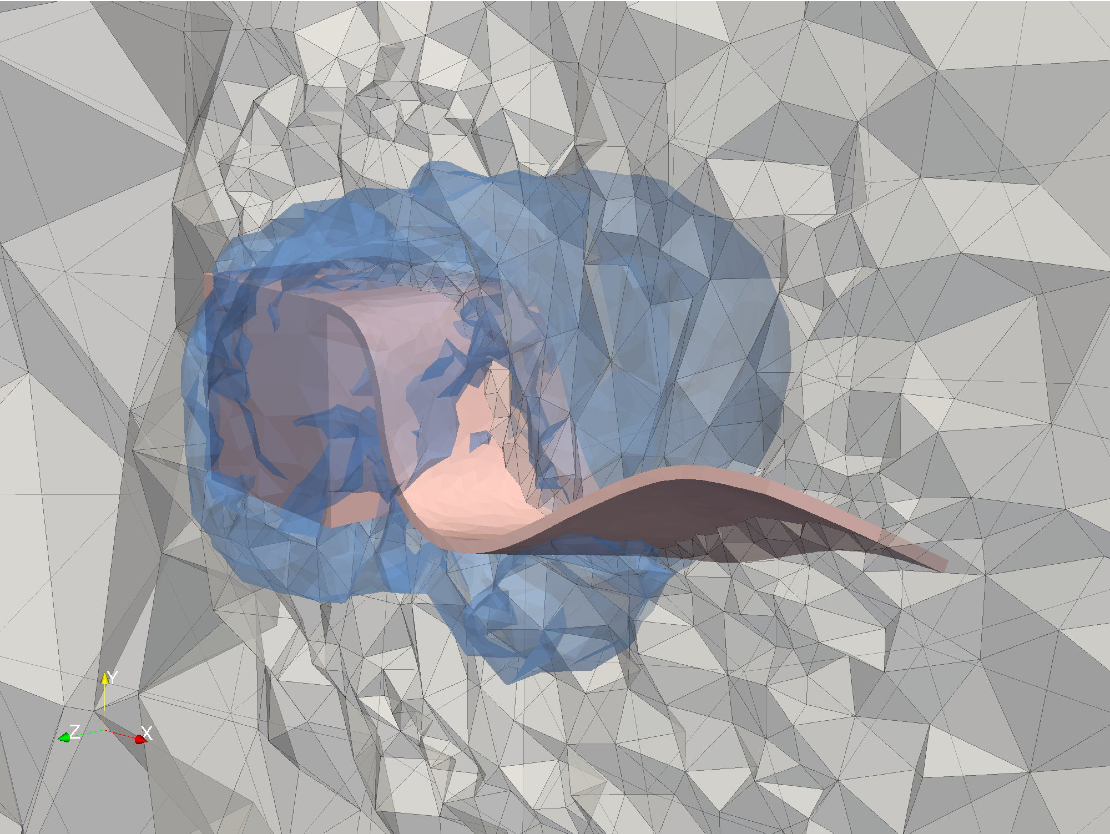
\includegraphics[width=5cm]{chapters/hoffman-1/png/cube168.png}\\
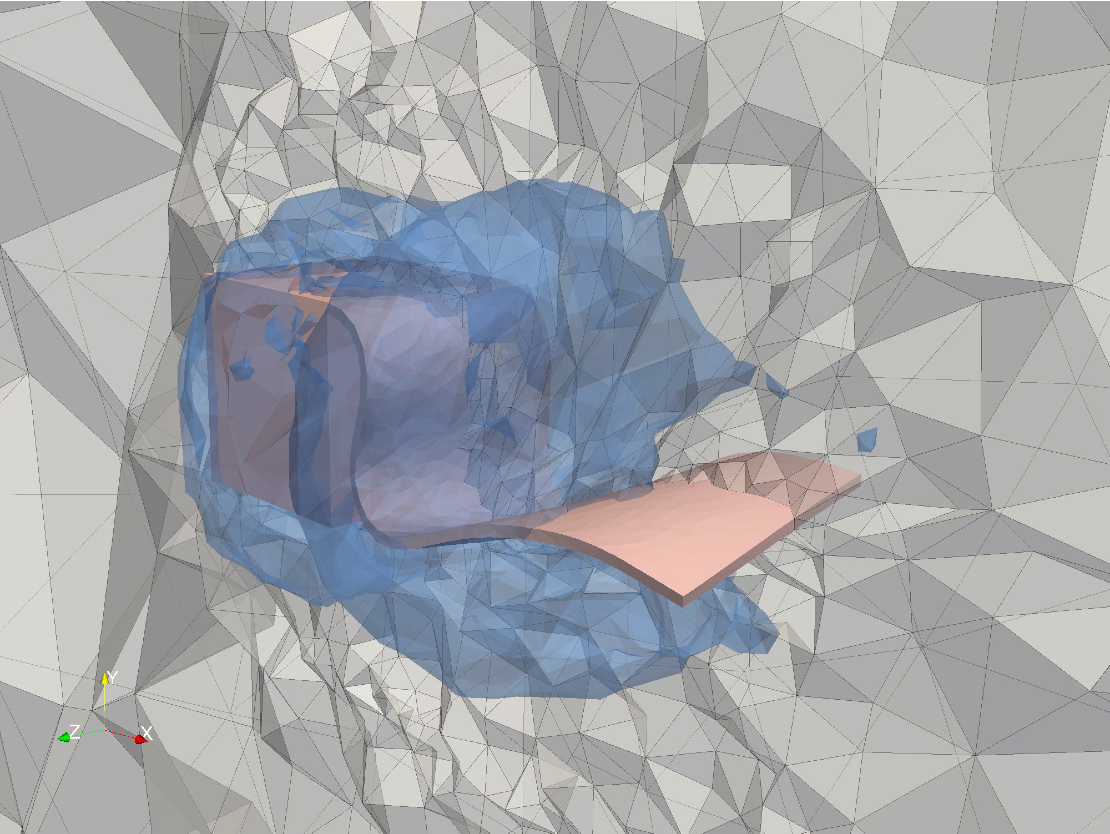
\includegraphics[width=5cm]{chapters/hoffman-1/png/cube187.png}
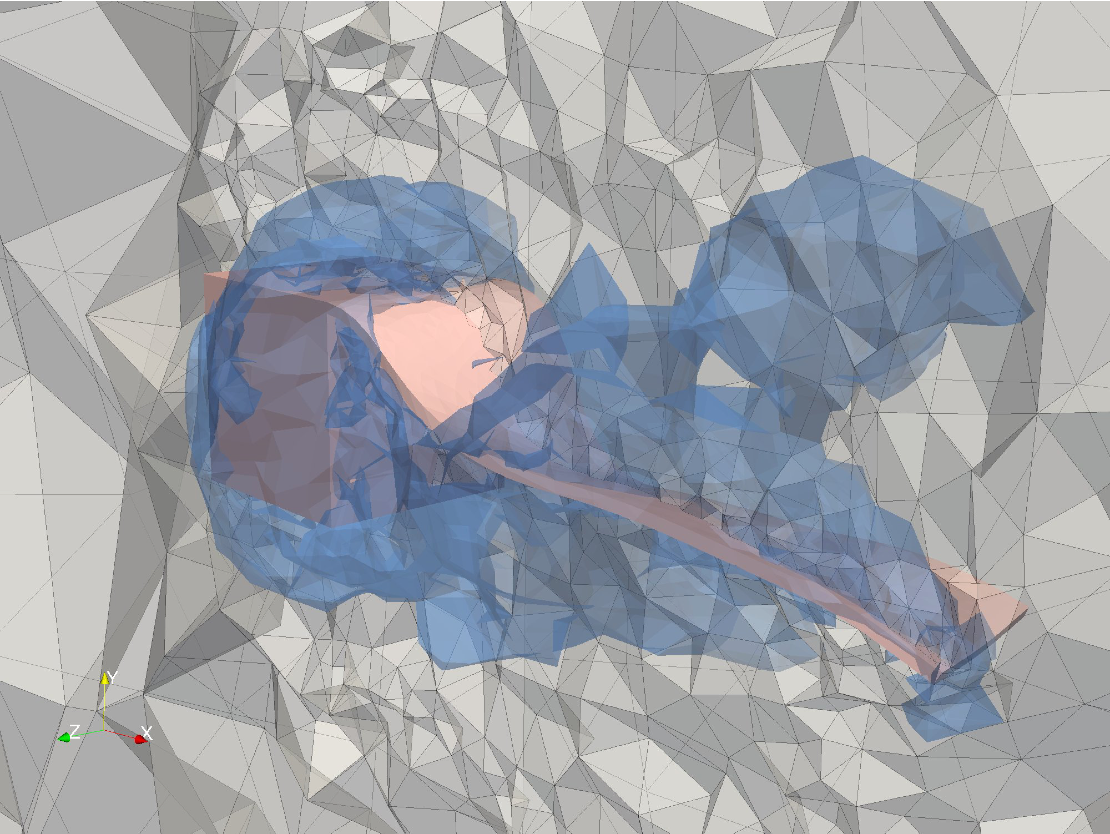
\includegraphics[width=5cm]{chapters/hoffman-1/png/cube405.png}\\
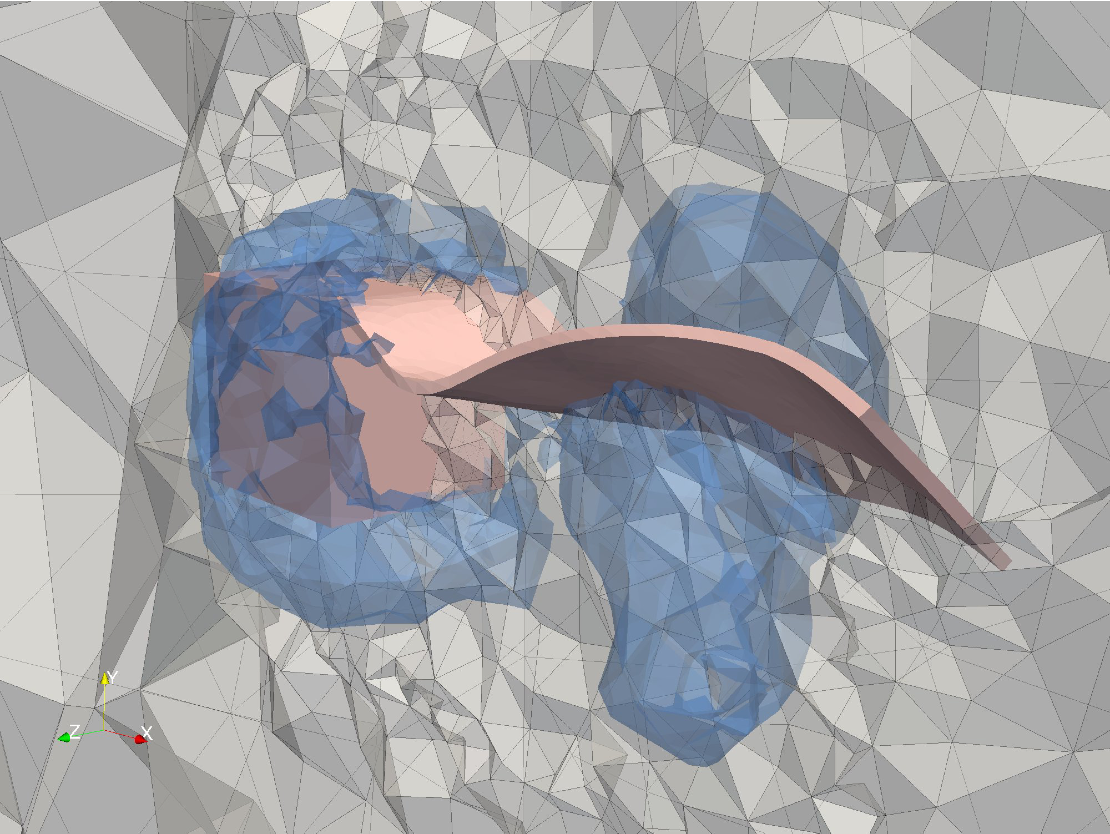
\includegraphics[width=5cm]{chapters/hoffman-1/png/cube550.png}
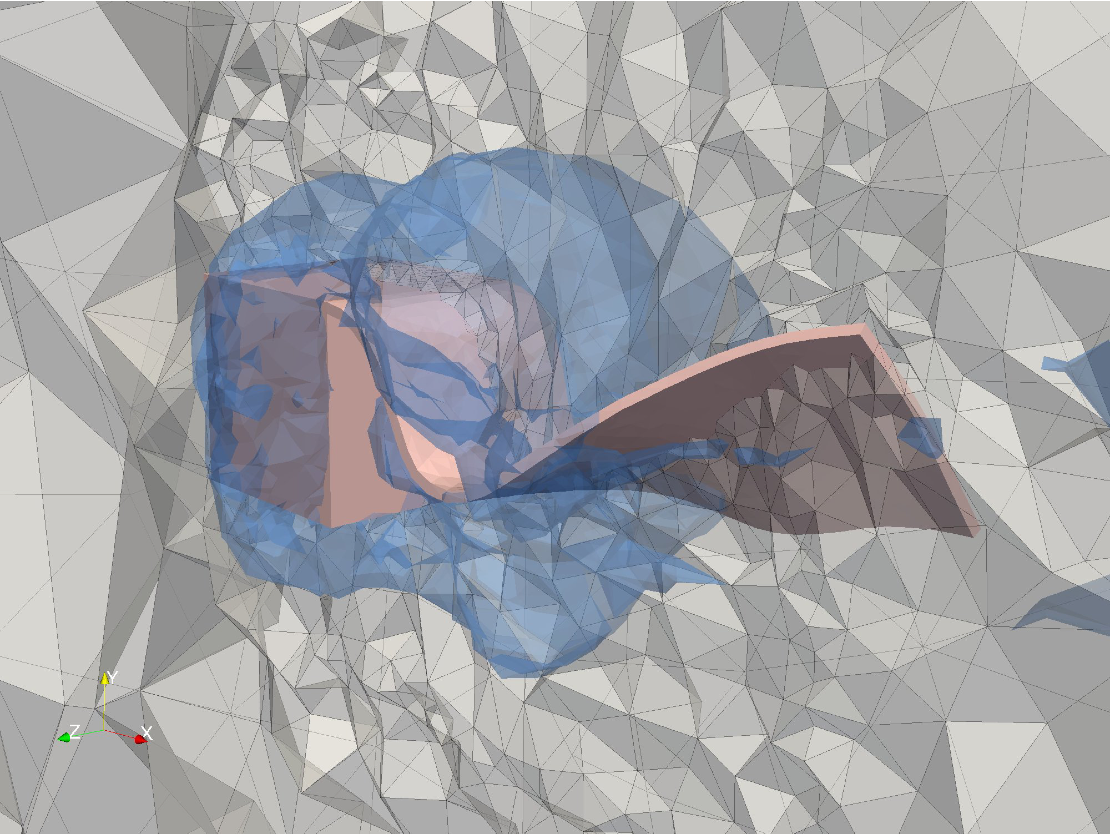
\includegraphics[width=5cm]{chapters/hoffman-1/png/cube649.png}\\
}
\caption{
Simulation of turbulent flow past a square cylinder with an elastic flag attached downstream \cite{HoffmanJanssonStockli2011}:
plot of cut of the mesh, isosurface of pressure and fluid--structure phase interface. Going from
initial state top left to illustrating violent bending and torsion
motion along the long axis of the flag.
}
\label{fig:flag}
\end{figure}


